\documentclass[uplatex,dvipdfmx,a4paper,11pt]{jsarticle}

\usepackage{docmute}


% 数式
\usepackage{amsmath,amsthm,amssymb}
\usepackage{bm}
% 画像
\usepackage{graphicx}

\usepackage{multirow}
\usepackage{wrapfig}
\usepackage{ascmac}
\usepackage{xcolor}


\usepackage{makeidx}
\makeindex

\graphicspath{{../../_Figures//}{../../_Figures/Rheology/}}

\usepackage{qrcode}
\setlength\lineskiplimit{0pt}
\setlength\normallineskiplimit{0pt}

\usepackage{qexam}

\usepackage{titlesec}
\titleformat*{\section}{\Large\bfseries}
\titleformat*{\subsection}{\large\bfseries}
\titleformat*{\subsubsection}{\normalsize\bfseries}
\titleformat*{\paragraph}{\normalsize\bfseries}

% ページ設定
% \pagestyle{empty}
% 高さの設定
\setlength{\textheight}{\paperheight}   % ひとまず紙面を本文領域に
\setlength{\topmargin}{-5.4truemm}      % 上の余白を20mm(=1inch-5.4mm)に
\addtolength{\topmargin}{-\headheight}  % 
\addtolength{\topmargin}{-\headsep}     % ヘッダの分だけ本文領域を移動させる
\addtolength{\textheight}{-40truemm}    % 下の余白も20mmに%% 幅の設定
\setlength{\textwidth}{\paperwidth}     % ひとまず紙面を本文領域に
\setlength{\oddsidemargin}{-5.4truemm}  % 左の余白を20mm(=1inch-5.4mm)に
\setlength{\evensidemargin}{-5.4truemm} % 
\addtolength{\textwidth}{-40truemm}     % 右の余白も20mmに
% 図と本文との間
%\abovecaptionskip=-5pt
%\belowcaptionskip=-5pt
%
% 全体の行間調整
% \renewcommand{\baselinestretch}{1.0} 
% 図と表
%\renewcommand{\figurename}{Fig.}
%\renewcommand{\tablename}{Tab.}
%

% \makeatletter 
% \def\section{\@startsection {section}{1}{\z@}{1.5 ex plus 2ex minus -.2ex}{0.5 ex plus .2ex}{\large\bf}}
% \def\subsection{\@startsection{subsection}{2}{\z@}{0.2\Cvs \@plus.5\Cdp \@minus.2\Cdp}{0.1\Cvs \@plus.3\Cdp}{\reset@font\normalsize\bfseries}}
% \makeatother 

\usepackage[dvipdfmx,%
 bookmarks=true,%
 bookmarksnumbered=true,%
 colorlinks=false,%
 setpagesize=false,%
 pdftitle={数式に頼らない直感的理解による材料設計のためのレオロジー⼊⾨},%
 pdfauthor={佐々木裕},%
 pdfsubject={},%
 pdfkeywords={レオロジー; 材料設計; }]{hyperref}
\usepackage{pxjahyper}

\usepackage{plext}

\usepackage{niceframe} 
\usepackage{framed}
\newenvironment{longartdeco}{%
  \def\FrameCommand{\fboxsep=\FrameSep \artdecoframe}%
  \MakeFramed {\FrameRestore}}%
 {\endMakeFramed}
 
\usepackage{siunitx}

\newcommand{\rmd}{\mathrm{d}}

\usepackage[inline]{showlabels}

\begin{document}
\section*{この章の内容}

この章では、いよいよレオロジーの主たる対象である粘性と弾性を併せ持った粘弾性という性質について議論を進めていきます。
具体的には、粘性と弾性についての基本的なモデルであるフック固体\index{ふっくこたい@フック固体}とニュートン流体\index{にゅーとんりゅうたい@ニュートン流体}をベースとして、
その組み合わせとして時間に伴い変化していく複雑な現象である粘弾性へとつなげていくことを⽬指します。

具体的に列記すると、以下のような事項となります。
\begin{boxnote}
    \begin{itemize}
        \item 粘性と弾性についての再確認
            \begin{itemize}
                \item 固体と液体の応答について振り返り、
                \item その組み合わせとして粘弾性
            \end{itemize} 
        \item 粘弾性のモデル化
            \begin{itemize}
                \item 粘弾性の単純なモデルをつくって、
                \item 応力緩和と緩和時間
            \end{itemize} 
        \item 少しだけ実事象に近づけると
            \begin{itemize}
                \item 複数の緩和時間を一般化マックスウェルモデルで
                \item 応力緩和で見た固体と液体
            \end{itemize}
    \end{itemize}
\end{boxnote}


\section{粘性\index{ねんせい@粘性}と弾性\index{だんせい@弾性}についての再確認}
まず、レオロジーのやり方についての再確認から始めていきましょう。

レオロジーとは、物質に刺激を与えてその応答を評価観察することで、その特性を評価する手法でした。
力学的な刺激を考えた場合、それに対する応答は、固体\index{こたい@固体}であれば弾性率という変形の容易さに応じた応力の発生であり、
また、流体\index{りゅうたい@流体}では粘度\index{ねんど@粘度}という指標で示される抵抗を持って流動\index{りゅうどう@流動}するというような応答が得られることになります。

そして、それぞれの特性についての評価が、比較的に単純なモデル(固体\index{こたい@固体}としてはバネモデル\index{ばねもでる@バネモデル}、液体\index{えきたい@液体}に対してはダッシュポットモデル\index{だっしゅぽっと@ダッシュポットモデル})
で表現できることをこれまでに示してきました。

しかしながら、実際の測定においては、それほど単純なわけでは有りません。
ここでは、レオロジーの主たる対象である粘性\index{ねんせい@粘性}と弾性\index{だんせい@弾性}を併せ持った粘弾性という性質についての議論へと進んでいきましょう。
\begin{figure}[htb]
	\begin{center}
		\begin{minipage}{0.4\textwidth}
			\begin{itemize}
				\item 力学的な刺激
				\begin{itemize}
					\item 外力による物質の変形
					\item あるいは、力の印加
				\end{itemize}
				\item 変形の結果として
				\begin{itemize}
					\item 固体として応力が発生
					\item 抵抗しながら流動
				\end{itemize}
				\item 弾性と粘性
			\end{itemize}
		\end{minipage}
		\begin{minipage}{0.5\textwidth}
			\begin{center}
			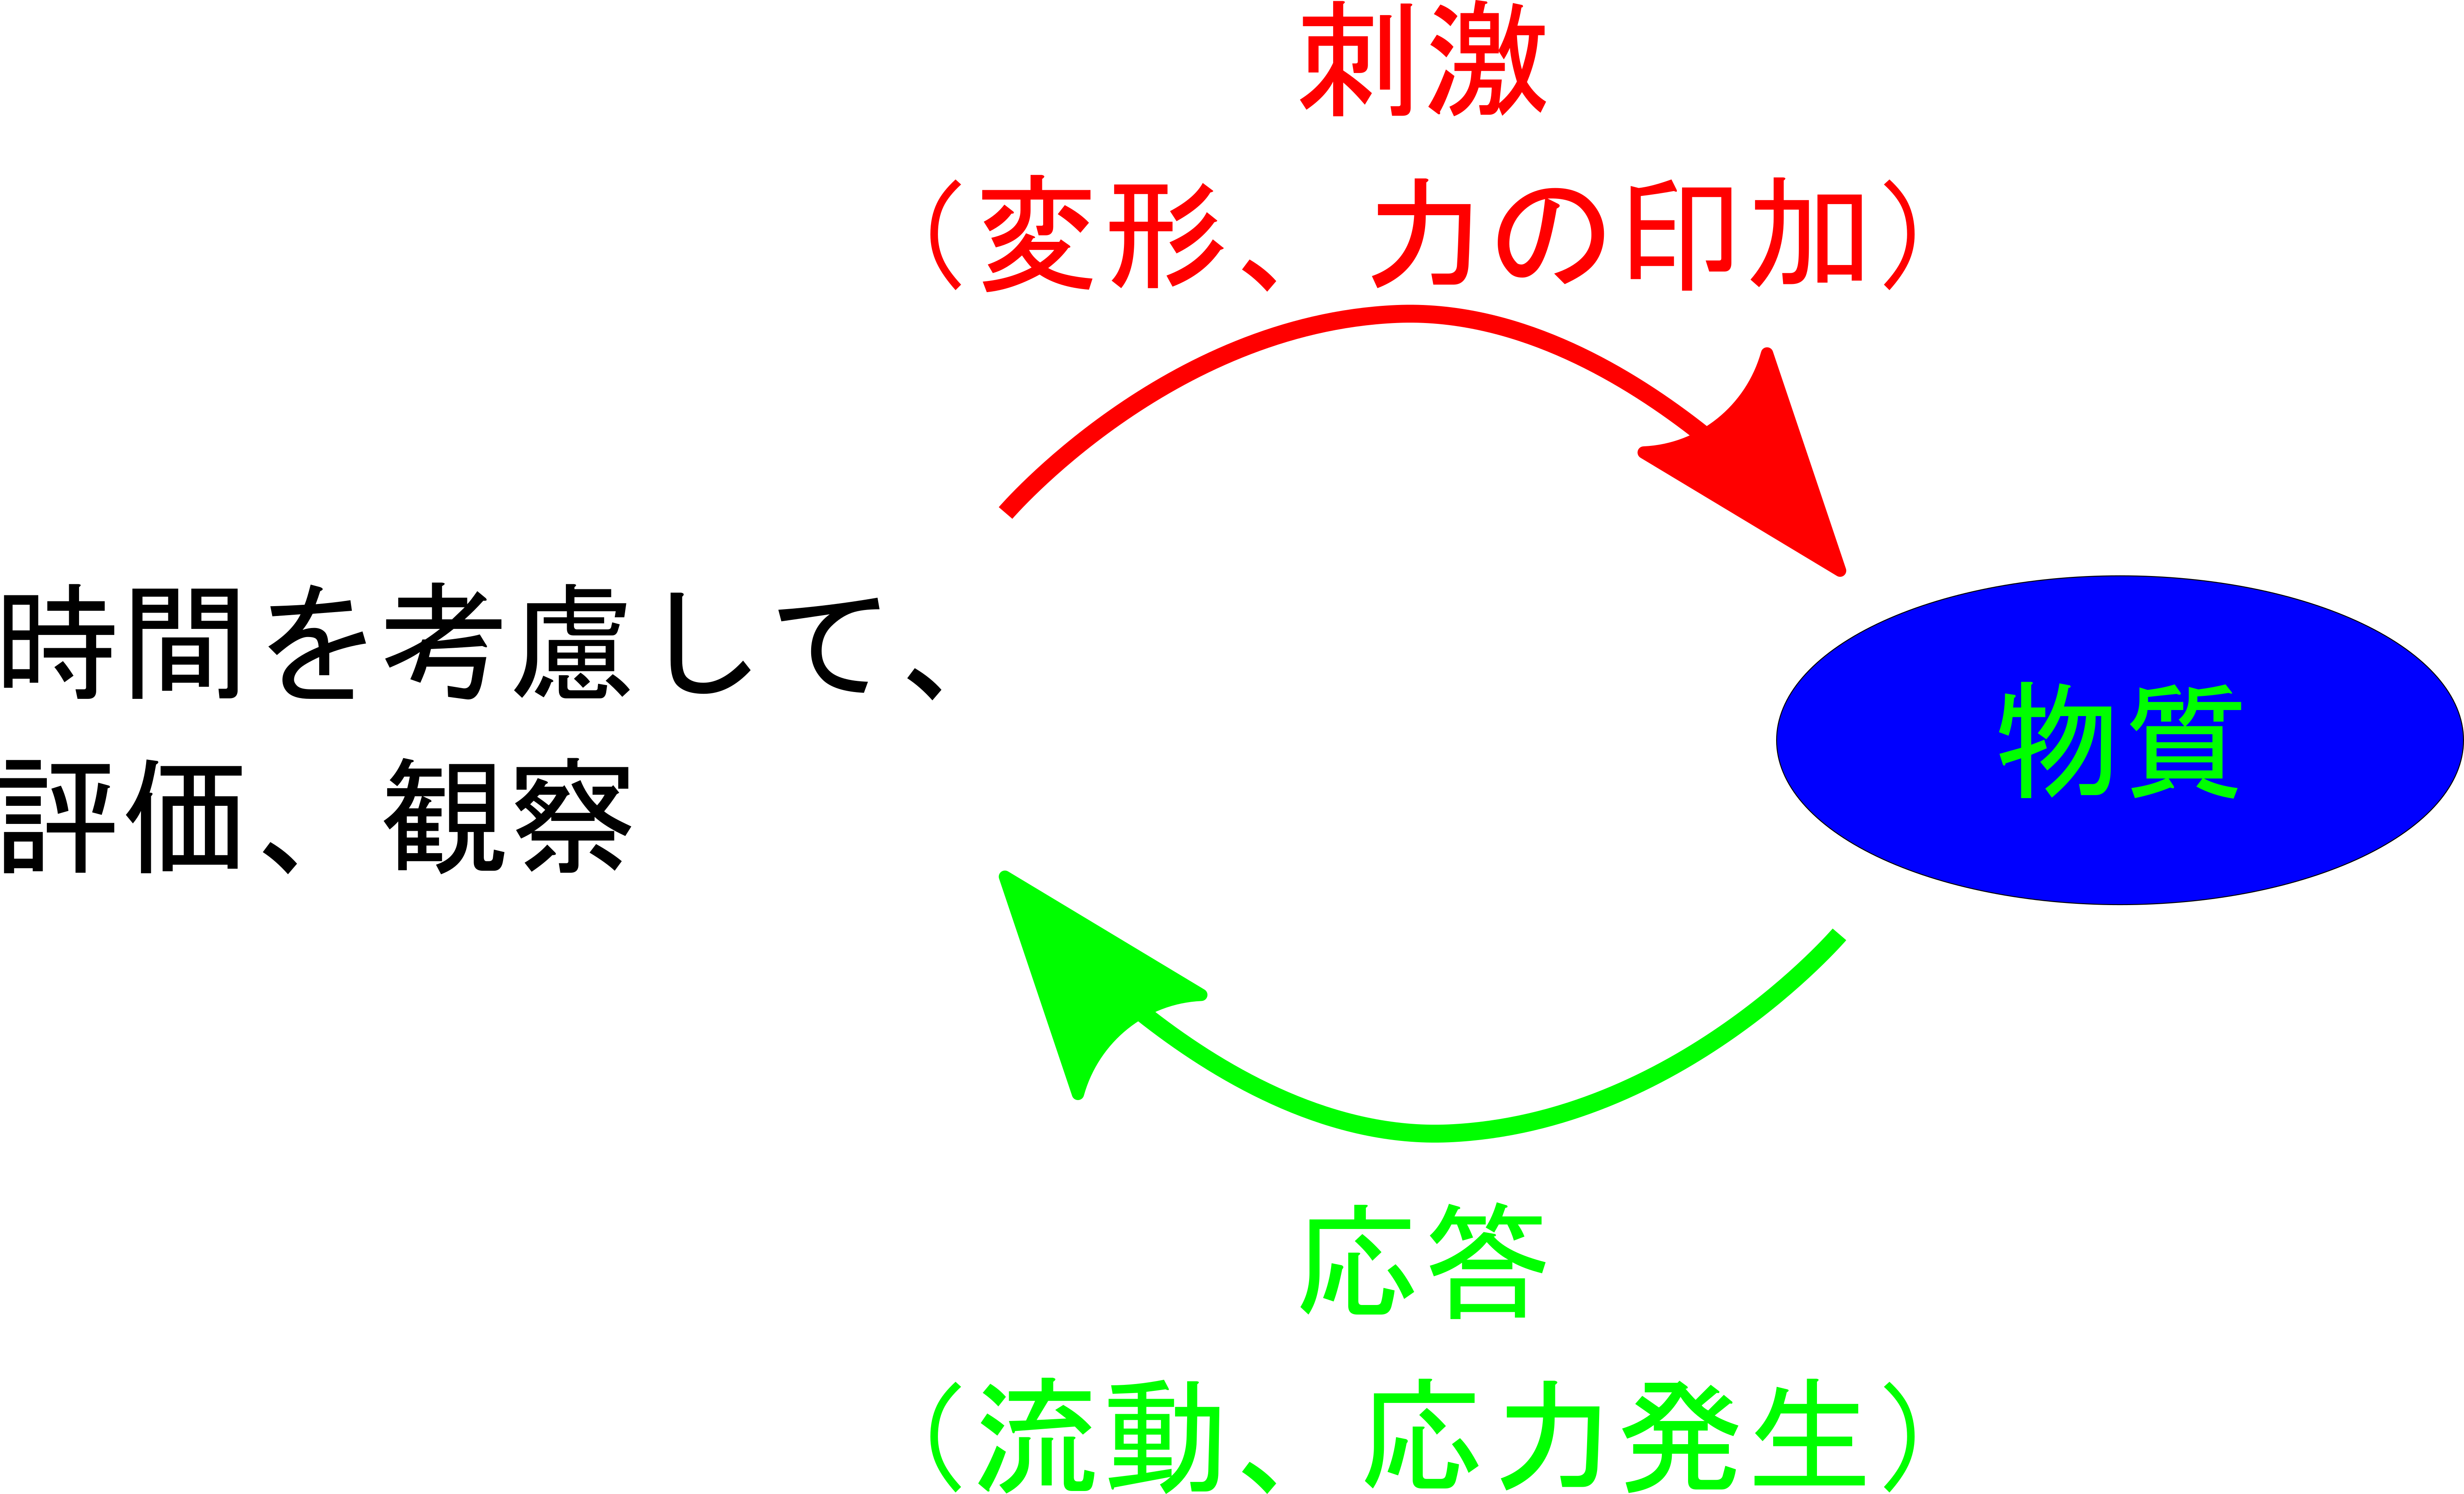
\includegraphics[width=\textwidth]{Rheo_method.png}
			\end{center}
		\end{minipage}
		\caption{レオロジーのやり方}
	\end{center}
\end{figure}

\subsection{固体\index{こたい@固体}と液体\index{えきたい@液体}の応答について}

固体と液体の応答について、再度簡単にまとめました。(表\ref{tab:kotaiekitai2})

\begin{table}[htb]
	\caption{固体と液体の応答}
	\label{tab:kotaiekitai2}
	\begin{center}
		\begin{tabular}{|c||c|} \hline
			固体のモデル & 液体のモデル \\ \hline \hline
			応力は\textcolor{red}{ひずみに比例} & 応力は\textcolor{red}{ひずみ速度\index{ひずみそくど@ひずみ速度}に比例}\\
			$\text{応力} = \text{弾性率} \times \text{ひずみ}$	& $\text{応力} = \text{粘度\index{ねんど@粘度}} \times \text{ひずみ速度}$ \\ \hline
			比例定数が弾性率\index{だんせいりつ@弾性率} & 比例定数が粘度\index{ねんど@粘度}\\ 
			弾性率の単位は、[Pa] & 粘度\index{ねんど@粘度}の単位は、[Pa$\cdot$s]\\ \hline
			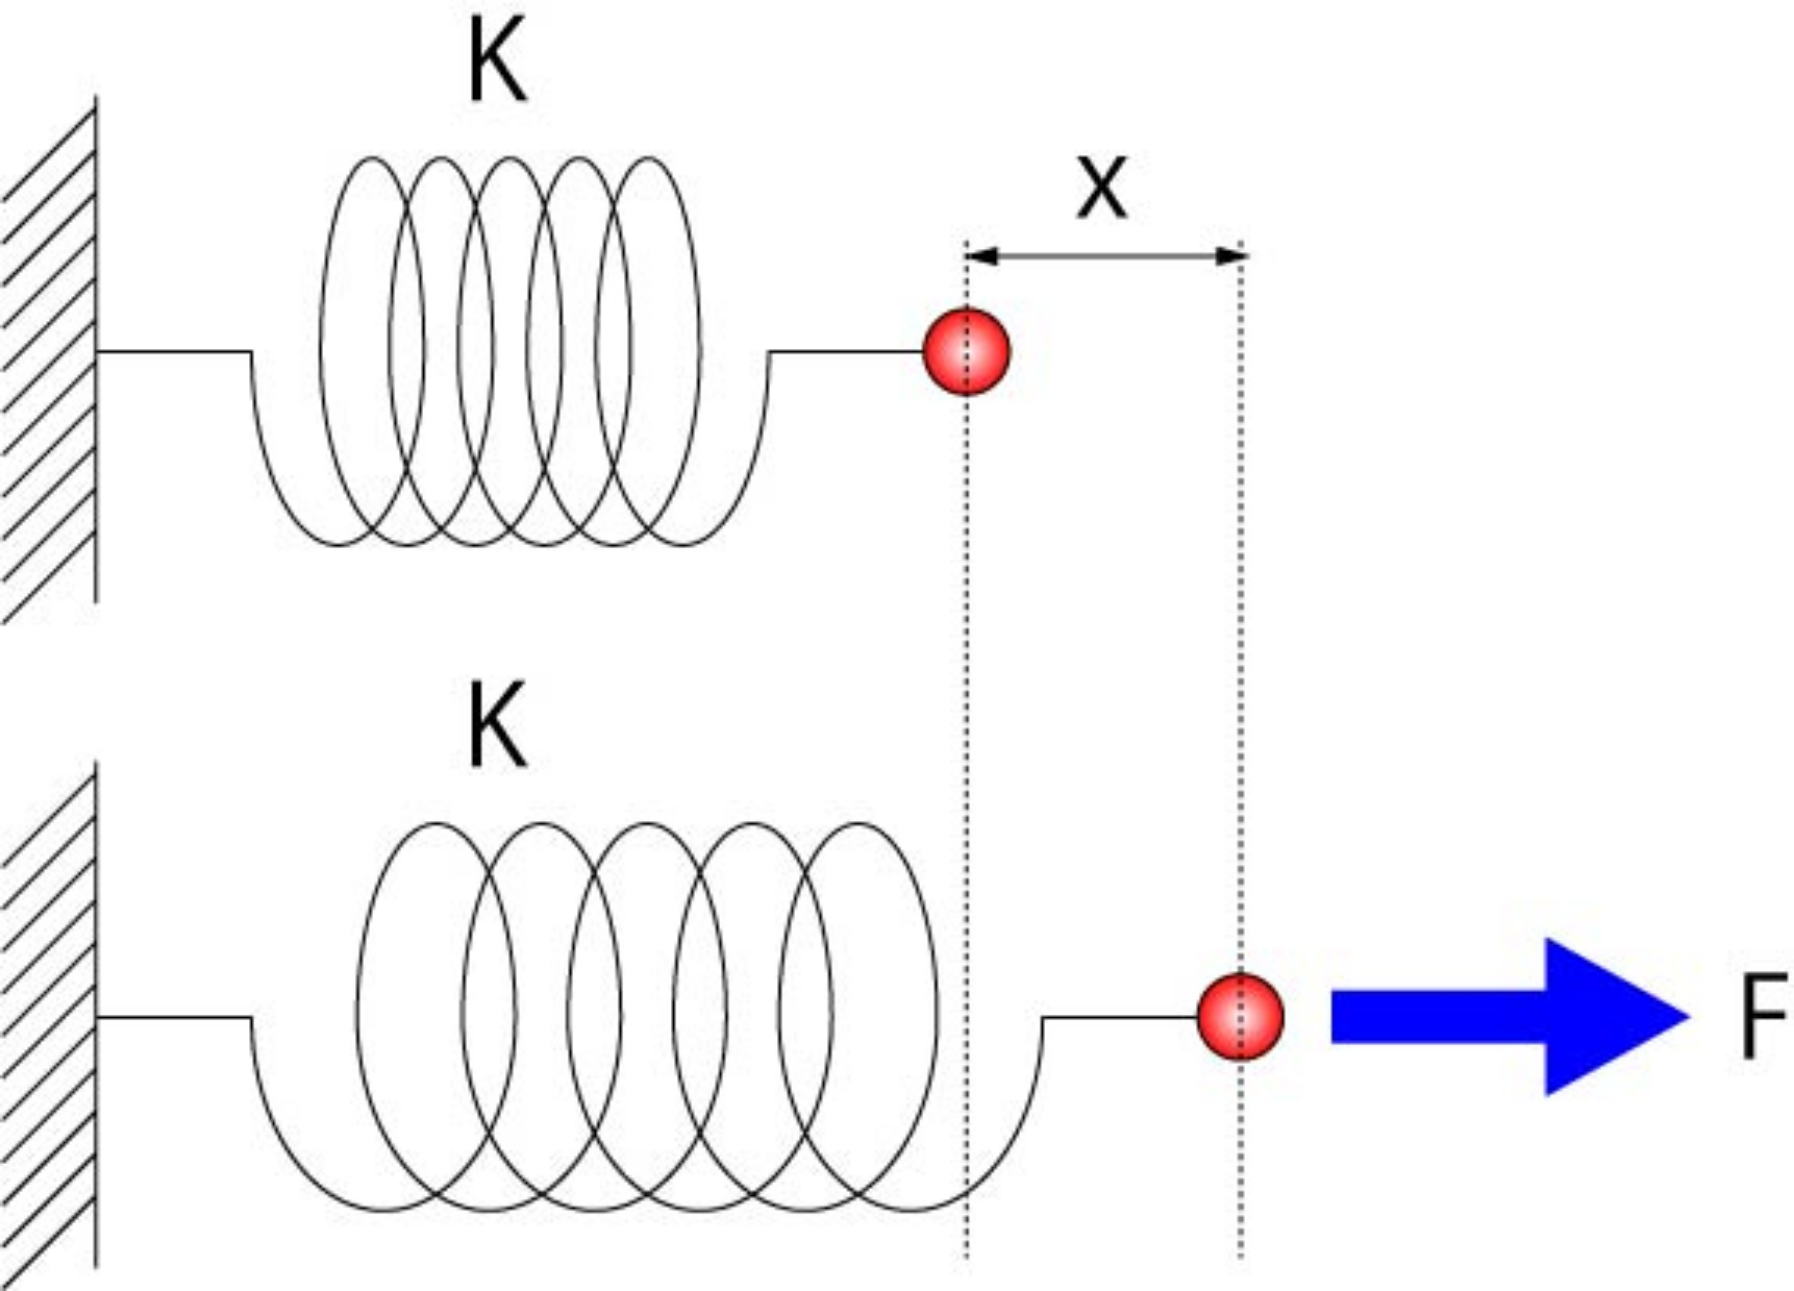
\includegraphics[width= 0.4\textwidth]{spring.png} & 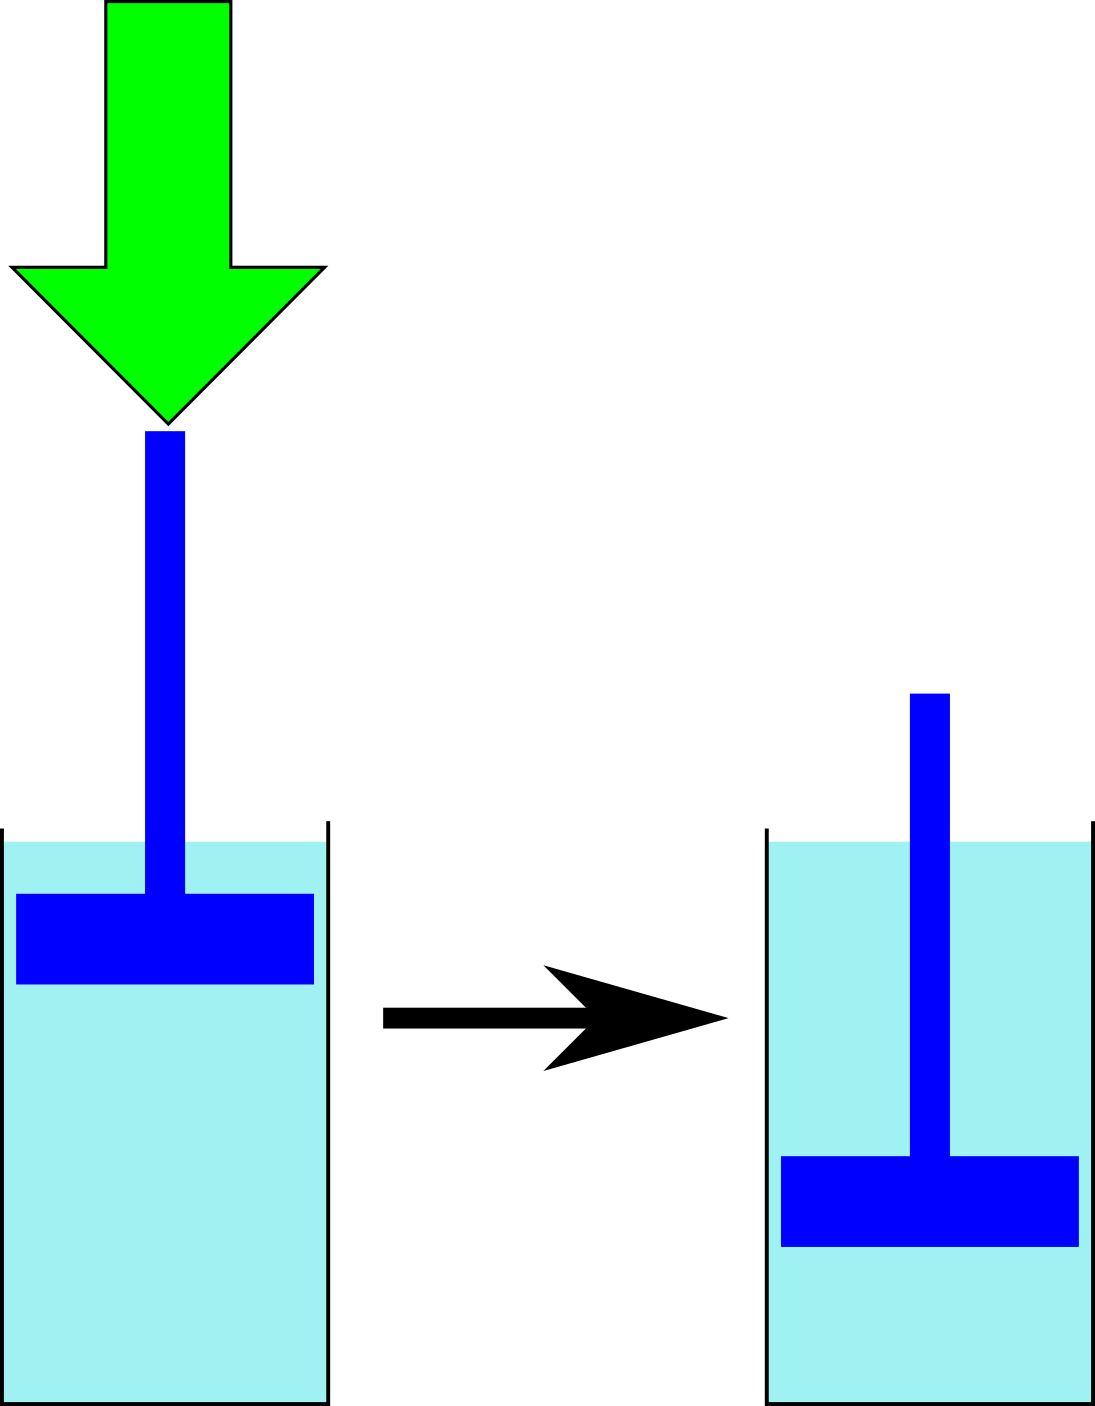
\includegraphics[width=.4\textwidth]{dashpot.png} \\ \hline
			\textcolor{red}{力の釣り合い} &  \textcolor{red}{時間の因子が重要} \\ \hline
		\end{tabular}
	\end{center}
\end{table}

固体\index{こたい@固体}において応力\index{おうりょく@応力}は付与した「ひずみ\index{ひずみ@ひずみ}」に比例するのですが、液体\index{えきたい@液体}では「ひずみ速度\index{ひずみそくど@ひずみ速度}」に比例することに注意してください。
固体\index{こたい@固体}では力の釣り合いという静的な現象として捉えることができますから、比較的単純に応答をイメージできることになります。
一方、流れるという応答においては時間の因子が重要になってきますので、その理解はそう単純ではなく複雑になってきます。

\subsection{実事象は複雑}
我々の身の回りにある実際の物質の応答は、固体\index{こたい@固体}と液体\index{えきたい@液体}とに簡単に二分されるわけでありません。

図 \ref{fig:outou_bingum} に、レオロジーという言葉の創始者であるビンガム先生が作成した、物質の力学的な応答について整理したものを示しました\footnote{
	Nature 1942 v149-3790, p702
}。

\begin{figure}[htb]
	\begin{center}
		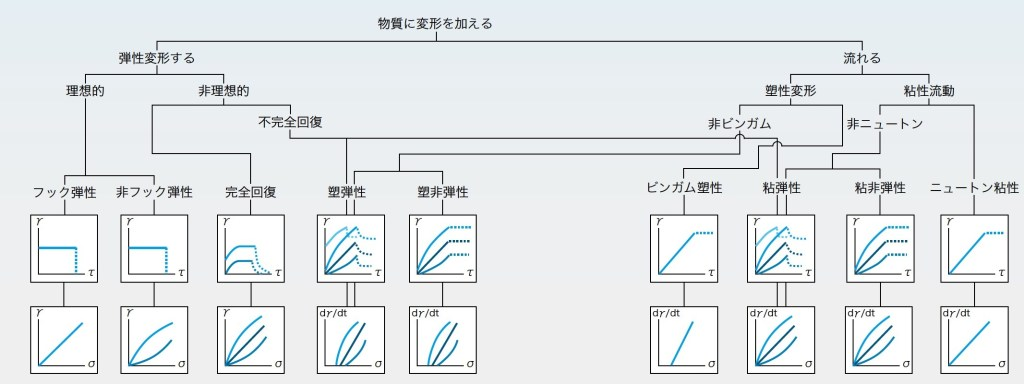
\includegraphics[width=.9\textwidth]{reoroji.jpeg}
		\caption{物質の力学的な応答}
		\label{fig:outou_bingum}
	\end{center}
\end{figure}

図の左半分が弾性変形という固体的な応答を示すグループであり、右側が流れるという液体\index{えきたい@液体}的な応答を示すグループに分けられています。
それらの中に、更に様々な応答挙動の分類がされています。

結局、我々の身の回りにある物質の力学的な応答は、固体と液体\index{えきたい@液体}と言うように単純に二分されるわけでもなく、
粘性\index{ねんせい@粘性}と弾性\index{だんせい@弾性}を併せ持ったものが多く存在することがわかります。

\subsection{粘弾性\index{ねんだんせい@粘弾性}について考えてみましょう}

では、ここから、粘性\index{ねんせい@粘性}と弾性\index{だんせい@弾性}を併せ持った、粘弾性\index{ねんだんせい@粘弾性}という性質について考えていきましょう。

物理モデルとしては、弾性\index{だんせい@弾性}を表すバネを用いたモデルと、粘性\index{ねんせい@粘性}を表すダッシュポットを用いたモデルとの、2つを組み合わせたモデルということになります。

\begin{figure}[htb]
	\begin{center}
		\begin{minipage}{0.4\textwidth}
			\begin{itembox}[l]{粘弾性という性質は?}
				\begin{itemize}
					\item 液体の流れる性質「粘性」と、
					\item 固体\index{こたい@固体}の変形する性質「弾性」を
					\item 合わせ持つ複雑な性質が、
					\item 「粘弾性」という性質です。
				\end{itemize}
			\end{itembox}
		\end{minipage}
		\begin{minipage}{0.45\textwidth}
			\begin{itembox}[l]{物理モデルとしては}
				\begin{itemize}
					\item 弾性を表すバネを用いたモデル
					\item 粘性を表すダッシュポットを用いたモデル
					\item 2つを組み合わせたモデル
				\end{itemize}
			\end{itembox}
		\end{minipage}
		\caption{粘弾性とは}
	\end{center}
\end{figure}

\section{粘弾性\index{ねんだんせい@粘弾性}のモデル化}

\subsection{粘弾性\index{ねんだんせい@粘弾性}の単純なモデル}
粘弾性\index{ねんだんせい@粘弾性}を物理モデルとして表現するときに基本となるものは、弾性\index{だんせい@弾性}を表すバネと粘性\index{ねんせい@粘性}を表すダッシュポットを直列に連結したモデルである
マックスウェルモデル\index{まっくすうぇるもでる@マックスウェルモデル}になります。

このモデルにおいては、外部からの刺激に対して、それぞれのユニットが錬成して応答することになります。
その内容について、詳しく考察していきましょう。

\begin{figure}[htb]
	\begin{center}
		\begin{minipage}{0.45\textwidth}
			\begin{itembox}[l]{マックスウェルモデルの数式}
				\begin{itemize}
					\item 弾性モデル
					\begin{align*}
						\sigma_s(t) = E \varepsilon_s(t)
					\end{align*}
					\item 粘性モデル
					\begin{align*}
						\sigma_d(t) = \eta \dfrac{\mathrm{d}}{\mathrm{d}t}\varepsilon_d(t)
					\end{align*}
					\item 直列に連結だから、
					\begin{itemize}
						\item 応力は共通
					\item ひずみはそれぞれの和
					\end{itemize}
				\end{itemize}	
			\end{itembox}
		\end{minipage}
		\begin{minipage}{0.45\textwidth}
			\begin{center}
			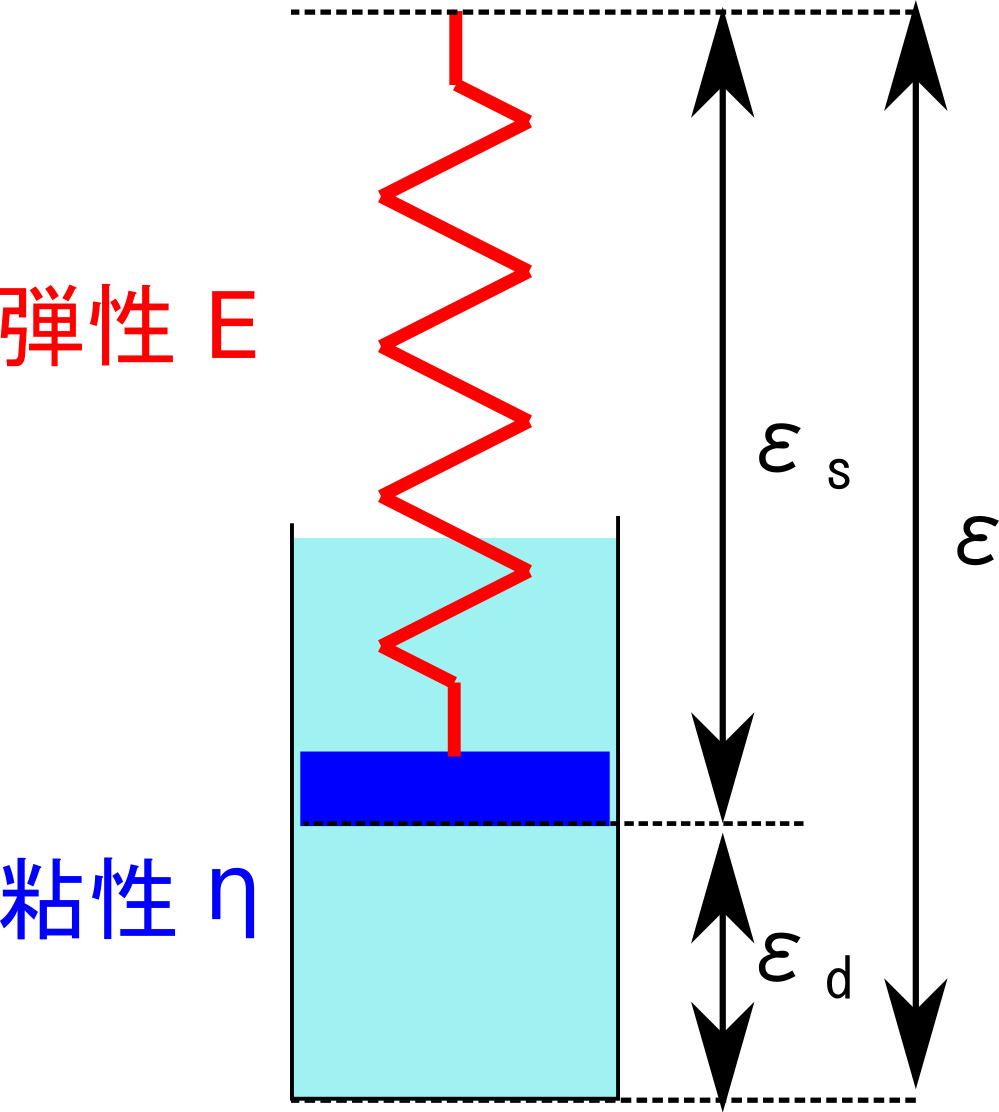
\includegraphics[width=.6\textwidth]{Maxwell_model.png}
			\end{center}
			\begin{align*}
				\begin{cases}
					\sigma = \sigma_s = \sigma_d \\
					\varepsilon = \varepsilon_s + \varepsilon_d
				\end{cases}
			\end{align*}
		\end{minipage}
		\caption{マックスウェルモデルとは}
		\label{fig:maxwell}
	\end{center}
\end{figure}

マックスウェルモデル\index{まっくすうぇるもでる@マックスウェルモデル}をそれぞれのユニットごとの表式の和として表し、「応力\index{おうりょく@応力}が共通」で、「ひずみ\index{ひずみ@ひずみ}はそれぞれのものの和」という二つの拘束条件を
考慮して解くと、図 \ref{fig:maxwell_eq} に示した微分方程式を得ることができます。
\begin{figure}[htb]
	\begin{center}
		\begin{minipage}{0.9\textwidth}
			\begin{itembox}[l]{マックスウェルモデルの数式について}
				$\varepsilon = \varepsilon_s + \varepsilon_d$ を微分して、
				\begin{align*}
					\dfrac{\mathrm{d}}{\mathrm{d}t}\varepsilon = \dfrac{\mathrm{d}}{\mathrm{d}t}\varepsilon_s + \dfrac{\mathrm{d}}{\mathrm{d}t}\varepsilon_d
				\end{align*}
				
				一方、弾性モデルの $\sigma_s(t) = E \varepsilon_s(t)$ を微分して、
				\begin{align*}
					\dfrac{\mathrm{d}}{\mathrm{d}t}\sigma = E \dfrac{\mathrm{d}}{\mathrm{d}t}\varepsilon_s
				\end{align*}
		
				これらを、粘性モデルの $\sigma_d(t) = \eta \dfrac{\mathrm{d}}{\mathrm{d}t}\varepsilon_d(t)$ に代入することで、
				以下に示した微分方程式として、\textcolor{red}{マックスウェルの方程式\index{まっくすうぇる@マックスウェルの方程式}}を得る。
				\color{red}
				\begin{align*}
					\dfrac{\mathrm{d}\varepsilon}{\mathrm{d}t} = \dfrac{1}{E} \dfrac{\mathrm{d}\sigma}{\mathrm{d}t} + \dfrac{\sigma}{\eta}
				\end{align*}
			\end{itembox}
		\end{minipage}
		\caption{マックスウェルの方程式}
		\label{fig:maxwell_eq}
	\end{center}
\end{figure}

\subsection{応力緩和\index{おうりょくかんわ@応力緩和}}

\subsubsection{応力緩和現象のイメージ}
粘弾性挙動を、直感的に理解できるような実験として、応力緩和\index{おうりょくかんわ@応力緩和}という実験があります。

これは、時刻 0 において、物質に瞬間的に歪を与えてそのまま保持します。
そうすると、付与したひずみに対応して物質中に生じていた応力が、時間の経過に従って、次第に減少(緩和\index{かんわ@緩和})していくという現象です。
イメージ図を、図 \ref{fig:stress_relux} に示しました。
\begin{figure}[htb]
	\begin{center}
		\begin{minipage}{0.45\textwidth}
			\begin{itembox}[l]{マクロな変形}
				\begin{itemize}
					\item 物質に、(瞬間的に)ひずみを与えて、
					\item その状態に維持。
					\item 応力が次第に減少。
				\end{itemize}
			\end{itembox}
		\end{minipage}
		\begin{minipage}{0.45\textwidth}
			\begin{center}
			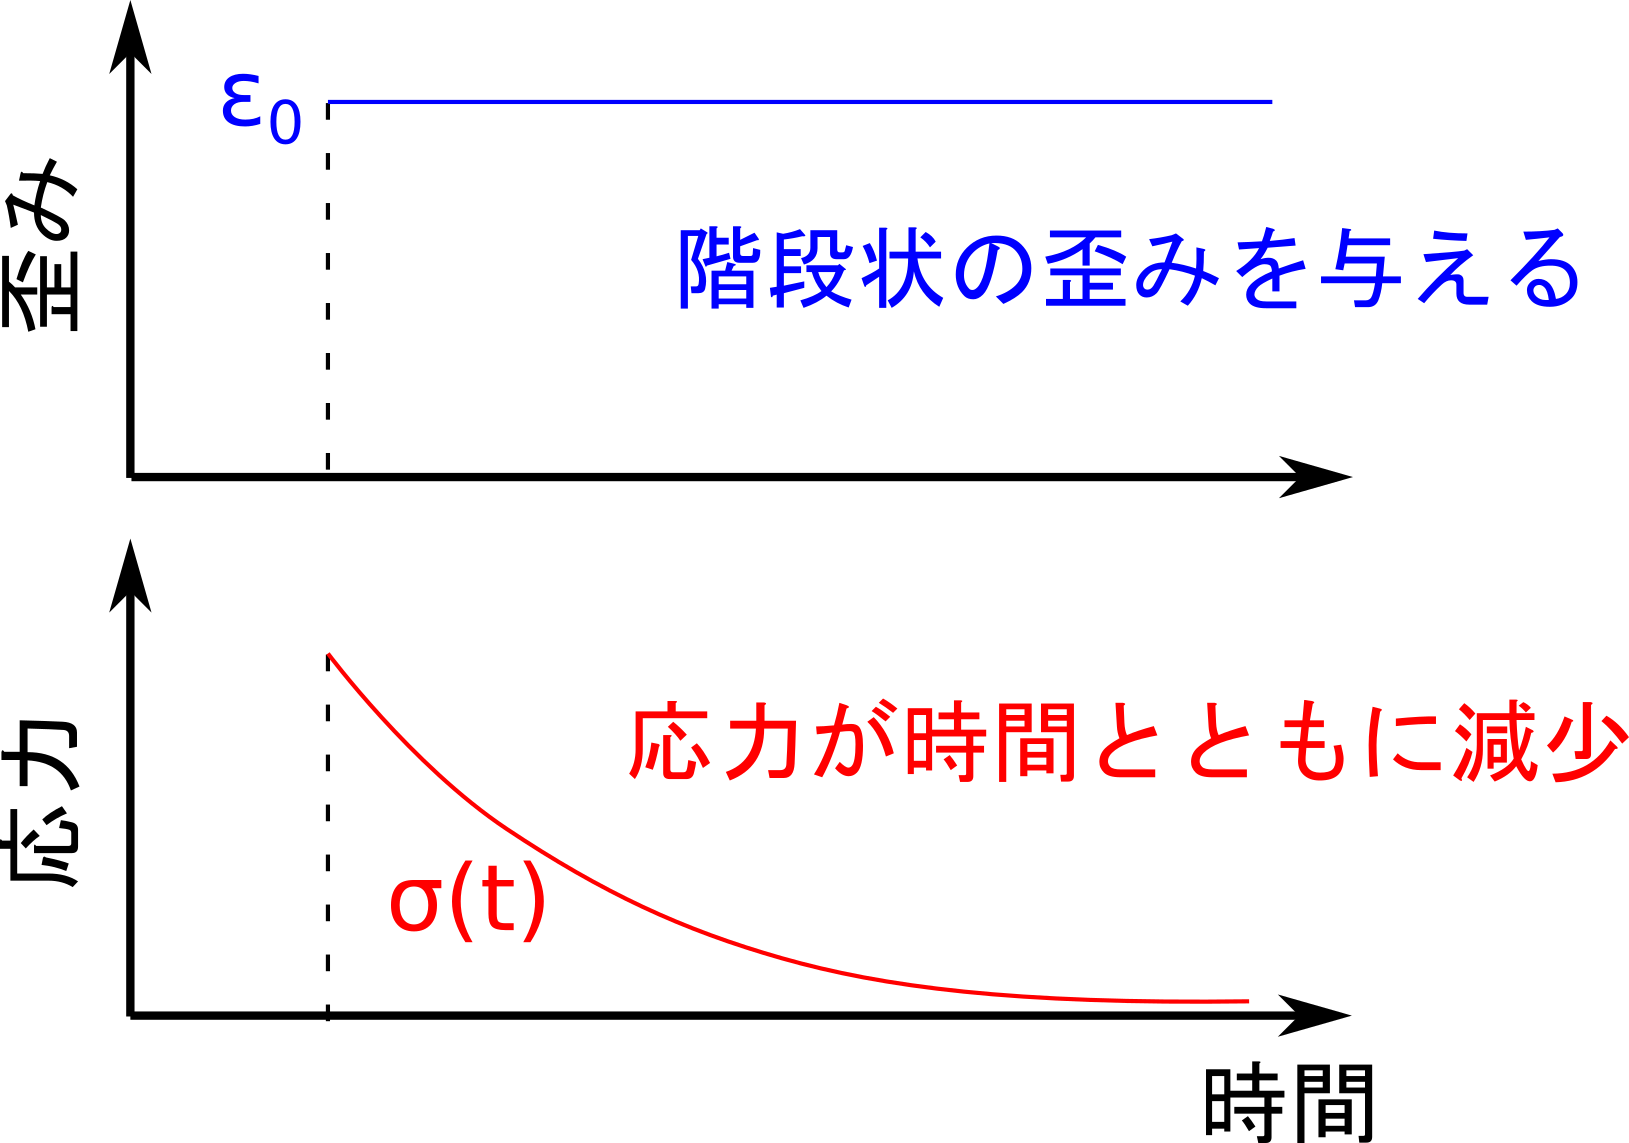
\includegraphics[width=.8\textwidth]{stress_relux.png}
			\end{center}
		\end{minipage}
		\caption{応力緩和}
		\label{fig:stress_relux}
	\end{center}
\end{figure}

この応力緩和現象は、ミクロには以下のように考えることができます。
\begin{center}
	\begin{minipage}{0.9\textwidth}
		\begin{itembox}[l]{ミクロに見た応力緩和現象}
			\begin{itemize}
				\item 巨視的な変形を受けたために、居心地のいい状態にいた粒子が、突然、居心地が変化。
				\item その環境下で、少しずつ、\textcolor{red}{居心地を改善}していく。
				\item その結果として、局所的な応力が消失し、その積分として\textcolor{red}{巨視的な応力が緩和}。
			\end{itemize}
		\end{itembox}
	\end{minipage}
\end{center}
つまり、物質の内部では、ほんのわずかですが、粒子\index{りゅうし@粒子}が居心地のいい状態へと移動することにより、巨視的な応力が少しずつ消失していくわけです。
この応力\index{おうりょく@応力}が次第に減少していく過程を、緩和していると表現します。
なお、緩和するという言葉自体は特殊な科学用語というわけでもなく、普段の生活においても使用しますし、その対象は応力だけには限りません。
癌による苦痛を和らげることも緩和ケアと呼びますし、
応力\index{おうりょく@応力}であれ、何であれ、任意の時刻に存在していたものが時間の経過に伴って、次第に霧のように消えていくことを緩和すると呼ぶわけです。

そして、粘弾性\index{ねんだんせい@粘弾性}という現象においては、緩和していく挙動を理解することにより物質の成り立ちや振る舞いを理解できることになります。


\subsubsection{マックスウェル方程式での応力緩和\index{おうりょくかんわ@応力緩和}}
応力緩和現象を、マックスウェル方程式を用いて解いていきましょう。

応力緩和\index{おうりょくかんわ@応力緩和}では、時刻 0 で瞬間的にひずみ\index{ひずみ@ひずみ}を印加して、その状態を保持します。
したがって、測定中はひずみ一定となりますので、ひずみ\index{ひずみ@ひずみ}の微分が 0 となります。
この条件をマックスウェル方程式に代入して、変数を移行した後に、両辺を積分します。

その後に、$t=0$ での初期応力 $\sigma_0$ を代入して変形します。
更に、対数\index{たいすう@対数}を指数\index{しすう@指数}に変換し、$\tau = \dfrac{\eta}{E}$ と書き換えて、応力緩和\index{おうりょくかんわ@応力緩和}に関する構成方程式を得ます。
\begin{align}
	\sigma(t) = \sigma_0 \exp \left(-\dfrac{t}{\tau} \right)
\end{align}

なお、ここで、突然現れた $\tau$ という変数の正体については後ほど議論しますが、指数\index{しすう@指数}関数の引数は無次元であるため、
分子と同じ時間の次元を持っていることだけは書いておきます。

\begin{figure}[htb]
	\begin{center}
		\begin{minipage}{0.9\textwidth}
			\begin{itembox}[l]{マックスウェル方程式で応力緩和を}
				応力緩和ではひずみ一定(ひずみの微分が 0)なので、$\dfrac{\mathrm{d}}{\mathrm{d}t}\varepsilon =0$ を
				マックスウェル方程式に代入して、
				\begin{align*}
					&\dfrac{1}{E} \dfrac{\mathrm{d}\sigma}{\mathrm{d}t} + \dfrac{\sigma}{\eta} = 0 \\
					&\dfrac{\mathrm{d}\sigma}{\mathrm{d}t} = -\dfrac{E}{\eta} \sigma \;\; 
					\text{\textcolor{blue}{(上式の第一項を右辺に移行)}}\\
					&{\color{red}\int \dfrac{1}{\sigma} \mathrm{d}\sigma} = -\dfrac{E}{\eta}  {\color{red} \int \mathrm{d}t} \; \;
					\text{\textcolor{blue}{(変数を振り分けてから、両辺を積分)}}\\
					&{\color{red}\ln \sigma} = -\dfrac{E}{\eta} {\color{red}t} + C \;\; 
					\text{\textcolor{blue}{(\textcolor{red}{積分の公式}に従い、積分定数を追加)}}
				\end{align*}

				$t=0$ での初期応力を $\sigma_0$ とすると、$C=\ln \sigma_0$ となり、
				\begin{align*}
					&\ln \sigma = -\dfrac{E}{\eta} t + \ln \sigma_0 \\
					&\ln \sigma - \ln \sigma_0 = -\dfrac{E}{\eta} t \\
					&\ln \dfrac{\sigma}{\sigma_0} = -\dfrac{E}{\eta} t \;\; \text{\textcolor{blue}{(対数の引き算は、真数の割り算)}}
				\end{align*}

				対数を指数\index{しすう@指数}に変換して、$\tau = \dfrac{\eta}{E}$ と書き換えて、

				\begin{align*}
					\sigma(t) = \sigma_0 \exp \left(-\dfrac{E}{\eta} t \right) = \sigma_0 \exp \left(-\dfrac{t}{\tau} \right)
				\end{align*}
			\end{itembox}
		\end{minipage}
		\caption{マックスウェル方程式で応力緩和}
		\label{}
	\end{center}
\end{figure}

\subsubsection{応力緩和の挙動}

図 \ref{fig:stress_relux3} に、マックスウェルの方程式\index{まっくすうぇる@マックスウェルの方程式}により導出した応力緩和挙動を表す式をグラフに表したものを示しました。

この式は、時刻 $t=0$ での初期応力 $\sigma_0$ が時間の経過とともになめらかに減少していく過程を表しています。
その減少過程を記述しているのが、指数\index{しすう@指数}関数 $\exp\left(-t/\tau \right)$ ということになります。

ここで、指数\index{しすう@指数}関数の性質を思い出すと、引数が -1 であるときに、$1/e$ になるわけでしたから、$\tau$ だけ時間が経過することにより 
$1/e$ がくり返し生じることが理解できるはずです\footnote{
	$2\tau$ 時間が経過したときには、指数関数の引数は -2 ですから、応力\index{おうりょく@応力}は $1/e^2$ に減少しています。
}。
したがって、指数関数に従って応力\index{おうりょく@応力}が減少していく過程を記述するのに、$\tau$ という時間の単位はとても便利に使えるわけです。
この $\tau$ を、緩和時間\index{かんわじかん@緩和時間}と呼びます。

\begin{figure}[htb]
	\begin{center}
		\begin{minipage}{0.45\textwidth}
			\begin{itembox}[l]{指数関数的減少とは}
				\begin{itemize}
					\item 下式をグラフに表すと、右図となる。
					\begin{align*}
						\sigma(t) = \sigma_0 \exp \left(-\dfrac{t}{\tau} \right)
					\end{align*}
					\item 時間経過に伴い応力が減少し $t = \tau$ において
					\begin{align*}
						\sigma(\tau) 
						&= \sigma_0 \exp(-1)\\ 
						&= \dfrac{\sigma_0}{e}
					\end{align*}
				\end{itemize}
			\end{itembox}
		\end{minipage}
		\begin{minipage}{0.48\textwidth}
			\begin{center}
			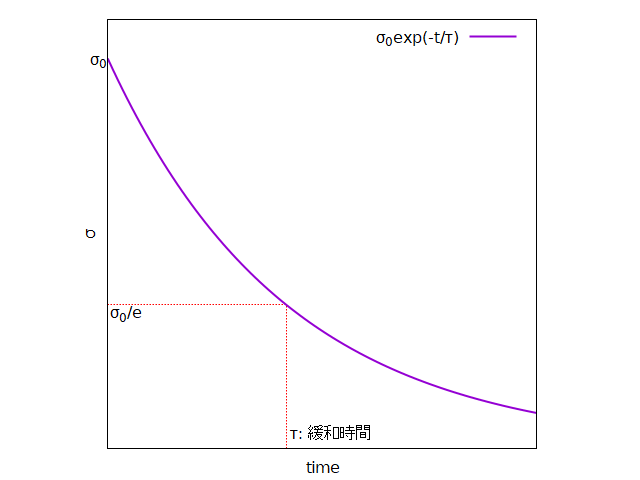
\includegraphics[width=\textwidth]{relux_3.png}
			\end{center}
		\end{minipage}
		\caption{応力緩和の挙動}
		\label{fig:stress_relux3}
	\end{center}
\end{figure}

\subsection{緩和時間\index{かんわじかん@緩和時間}}
緩和時間\index{かんわじかん@緩和時間}について、もう少し詳しく考察を勧めましょう。

\subsubsection{緩和時間\index{かんわじかん@緩和時間}について}
マックスウェル方程式からの式展開においては、粘度\index{ねんど@粘度} $\eta$ と弾性率\index{だんせいりつ@弾性率} $E$ との比として緩和時間\index{かんわじかん@緩和時間} $\tau$ を定義しましたから、
このことからも時間の単位を持つことは理解できます。
そして、弾性率\index{だんせいりつ@弾性率}という固体\index{こたい@固体}の特徴を表す比例定数と、粘度\index{ねんど@粘度}という液体\index{えきたい@液体}の特徴を表すものとの比ですから、
注目している物質の特徴が、固体的であるか、あるいは、液体的であるかという度合いを表現していると捉えることもできるわけです。

\begin{figure}[htb]
	\begin{center}
		\begin{minipage}{0.9\textwidth}
			\begin{itembox}[l]{緩和時間とは}
				\begin{align*}
					\text{(緩和時間)}\;\tau = \dfrac{\eta}{E}\; \left( \dfrac{\text{粘度\index{ねんど@粘度}}}{\text{弾性率}} \right)
				\end{align*}
				\begin{itemize}
					\item 緩和時間とは
					\begin{itemize}
						\item 弾性モデルにおける弾性率 $E$ の単位は Pa、
						\item 粘性\index{ねんせい@粘性}モデルにおける粘度\index{ねんど@粘度} $\eta$ の単位は Pa$\cdot$s、
						\item その比である $\tau$ は時間の次元 [T] を持ち、緩和時間と呼ばれる。
						\item 緩和時間とは、物質のひずみに対する力学応答が、指数関数的に減少するさまを表す特徴的な時間。
					\end{itemize}
					\item 緩和時間の振る舞い
					\begin{itemize}
						\item 弾性応答の性質を表す弾性率に反比例し、
						\item 粘性\index{ねんせい@粘性}応答の度合いを表す粘度\index{ねんど@粘度}に比例する。
						\item 注目している物質の特徴が、固体的であるか、あるいは、液体的であるかという度合いを表現
					\end{itemize}
				\end{itemize}
			\end{itembox}
		\end{minipage}
		\caption{緩和時間について}
		\label{fig:tau}
	\end{center}
\end{figure}

\subsubsection{対数プロット}
緩和時間\index{かんわじかん@緩和時間}の視覚的なイメージを持つためには、対数プロット\index{たいすう@対数プロット}も非常に有効です。

図 \ref{fig:log_plot_relux} に、片対数プットと両対数プロットを合わせて示しました。
プロットする軸のスケールのとり方で、見た目も大きく変化することがわかります。
\begin{figure}[htb]
	\begin{center}
		\begin{minipage}{0.45\textwidth}
			\begin{center}
				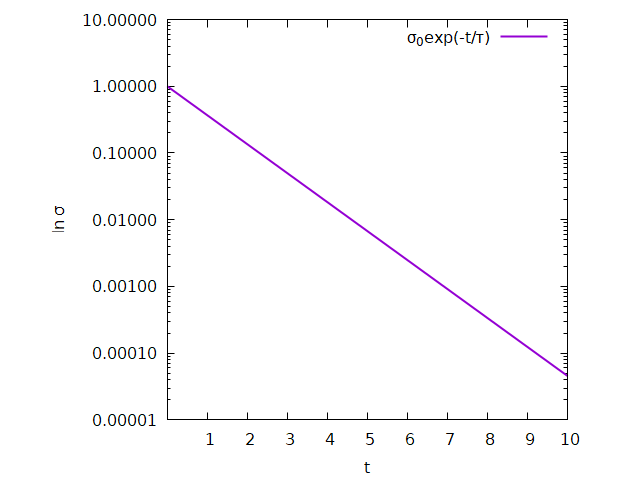
\includegraphics[width=\textwidth]{relux_4.png}

				片対数グラフ:\\傾きが緩和時間に対応
			\end{center}
		\end{minipage}
		\begin{minipage}{0.45\textwidth}
			\begin{center}
				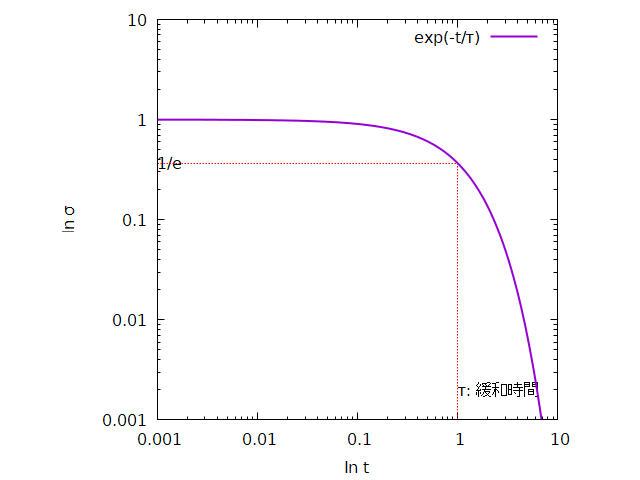
\includegraphics[width=\textwidth]{relux_5.png}

				両対数グラフ:\\緩和時間近傍で応力が急激に低下
			\end{center}
		\end{minipage}
		\caption{応力緩和関数の対数プロット}
		\label{fig:log_plot_relux}
	\end{center}
\end{figure}

片対数グラフ\index{かたたいすう@片対数グラフ}にプロットした場合には、傾きが緩和時間\index{かんわじかん@緩和時間}に対応することになります。
一方、両対数グラフ\index{りょうたいすう@両対数グラフ}では、緩和時間\index{かんわじかん@緩和時間}の少し前まではグラフの変化は非常に小さいものであり、
緩和時間近傍で応力\index{おうりょく@応力}が急激に低下するような挙動を見せることがわかります。

なお、注意していただきたいのは、対数プロットしたからと言って事象が変化しているわけではなくて、
その見え方が異なっているだけだということです。

\section{少しだけ実事象に近づけると}

前節では、マックスウェルモデル\index{まっくすうぇるもでる@マックスウェルモデル}という非常に単純なモデルであっても、一応、粘弾性\index{ねんだんせい@粘弾性}という挙動を表現することが可能であることを示しました。

緩和時間\index{かんわじかん@緩和時間}という特徴的な時間を用いることで、物質が固体的であるのか、液体的であるのかという粘弾性体としての特徴をざっくり分類することはできそうです。
しかしながら、実際の物質は、マックスウェルモデルだけで記述できるほど単純なわけは有りません。
ここでは、マックスウェルモデル\index{まっくすうぇるもでる@マックスウェルモデル}を応用することで、もう少しだけ実事象に近づけていくことを検討してみます。

\subsection{複数の緩和時間\index{かんわじかん@緩和時間}}
実際の物質の内部は、大抵の場合、均一とは言えないことが多い\footnote{
	材料力学等においては、問題の簡略化のために、均質な連続体モデルとして記述する場合が多く、弾性体についてはそれで十分となります。
	しかしながら、粘弾性体においては、そのような記述は理解の妨げになるかもしれません。
}わけであり、その結果として、マクロには複雑な緩和挙動を示すことになります。

ここで、仮想的に、物質の内部に複数の緩和時間\index{かんわじかん@緩和時間}があるようなモデルを考えてみると、
図 \ref{fig:relux_multi} のようにモデル化して考えることができます。
% なお、ここでは、単純化したモデルを作るために、緩和時間を離散的に数で数えられるようなものとして空間的に記号を表しましたが、
% 本当に物質中にそんな物があると勘違いしないように注意してください。
% この図はあくまでも仮想的なモデルであり、実際の物質中の、例えば、ポリマー鎖のようなものに対応するわけでは決して有りません。

\begin{figure}[htb]
	\begin{center}
		\begin{minipage}{0.45\textwidth}
			\begin{itembox}[l]{複数の緩和時間}
				\begin{itemize}
					\item 実際の物質の内部は、大抵の場合、均一とは言えないことが多い。
					\item その結果として、マクロには複雑な緩和挙動を示す。
					\item \textcolor{red}{仮想的}に、内部に\textcolor{red}{複数の緩和時間}を考えよう。
					\item 右図のように\textcolor{red}{モデル化}できる。
				\end{itemize}
			\end{itembox}
		\end{minipage}
		\begin{minipage}{0.45\textwidth}
			\begin{center}
			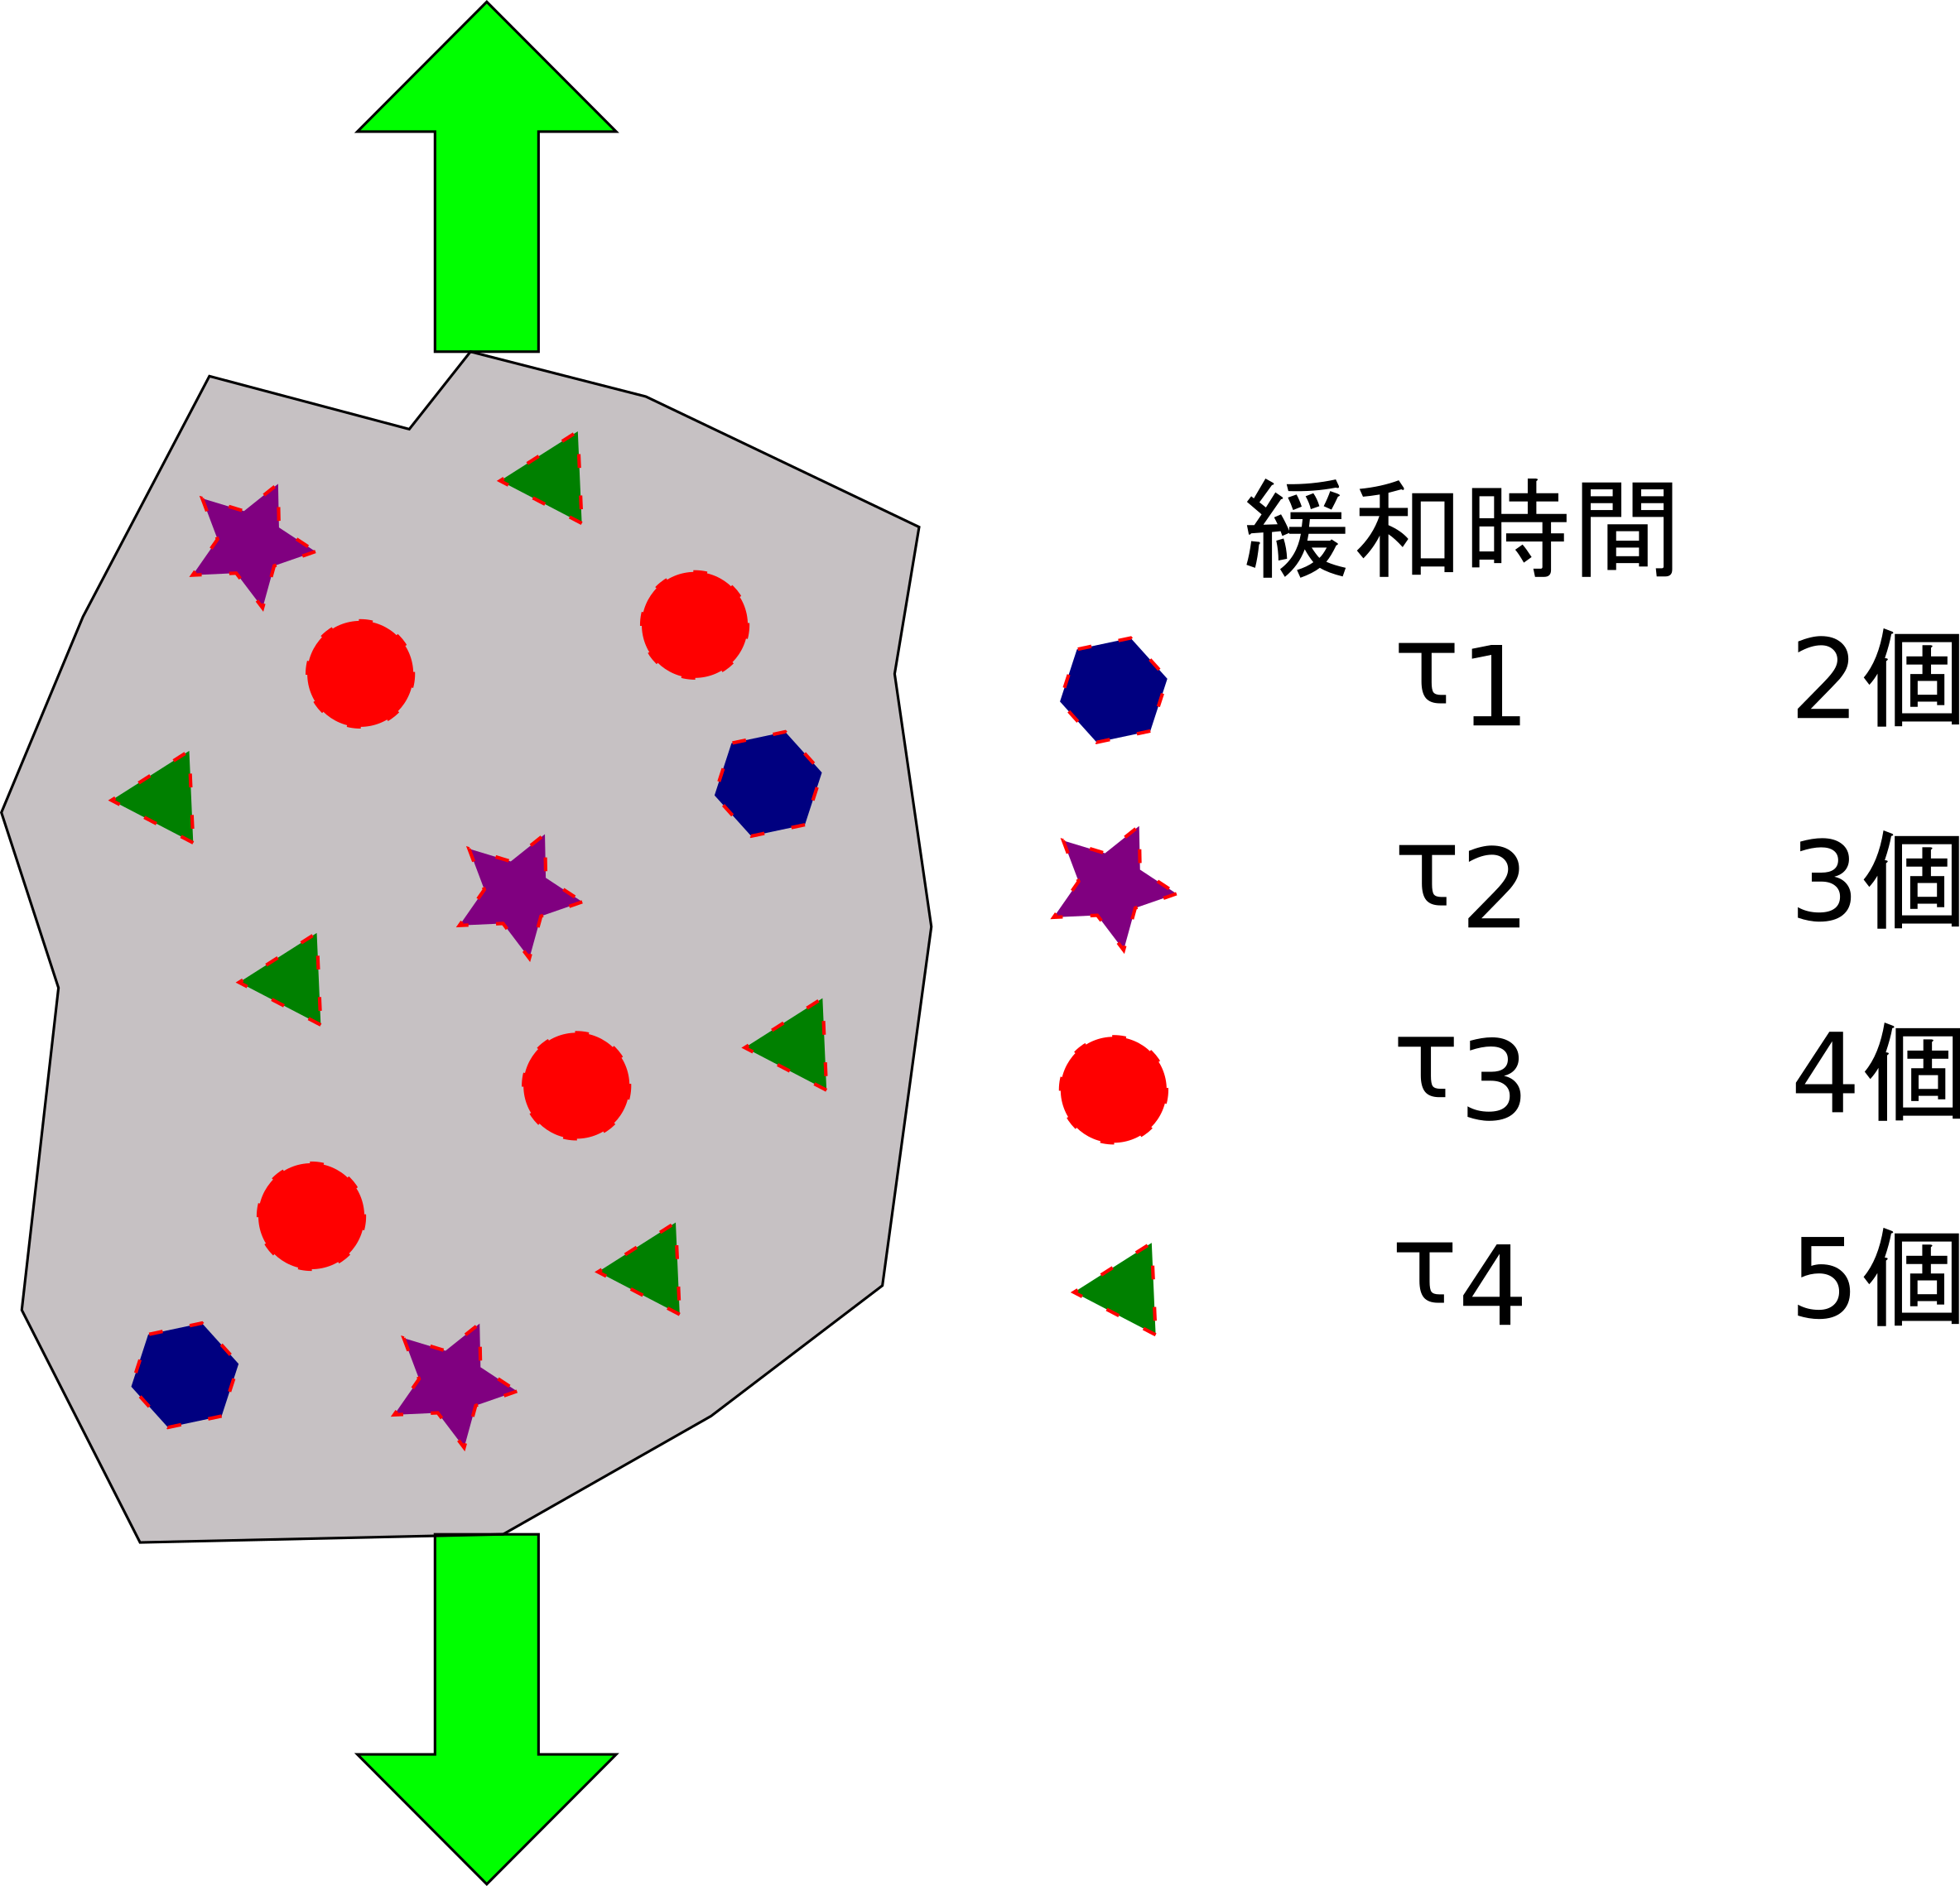
\includegraphics[width=.8\textwidth]{relux_multi.png}
			\end{center}
		\end{minipage}
		\caption{実際の物質中の複数の緩和時間}
		\label{fig:relux_multi}
	\end{center}
\end{figure}

\subsection{一般化マックスウェルモデル\index{いっぱんかまっくすうぇるもでる@一般化マックスウェルモデル}について}
前述のように、物質中に複数の緩和時間\index{かんわじかん@緩和時間}が存在するようなモデルを考えたとします。

それぞれの緩和時間\index{かんわじかん@緩和時間}に対応するように緩和時間\index{かんわじかん@緩和時間}の異なる複数のマックスウェルモデル\index{まっくすうぇるもでる@マックスウェルモデル}を想定して、
すべてを並列に連結したモデルを一般化マックスウェルモデル\index{いっぱんかまっくすうぇるもでる@一般化マックスウェルモデル}と呼びます。

\subsubsection{一般化マックスウェルモデルのイメージ図}
イメージ図として、図 \ref{fig:gen_maxwell} に示しました。
\begin{figure}[htb]
	\begin{center}
		\begin{minipage}{0.9\textwidth}
			\begin{center}
			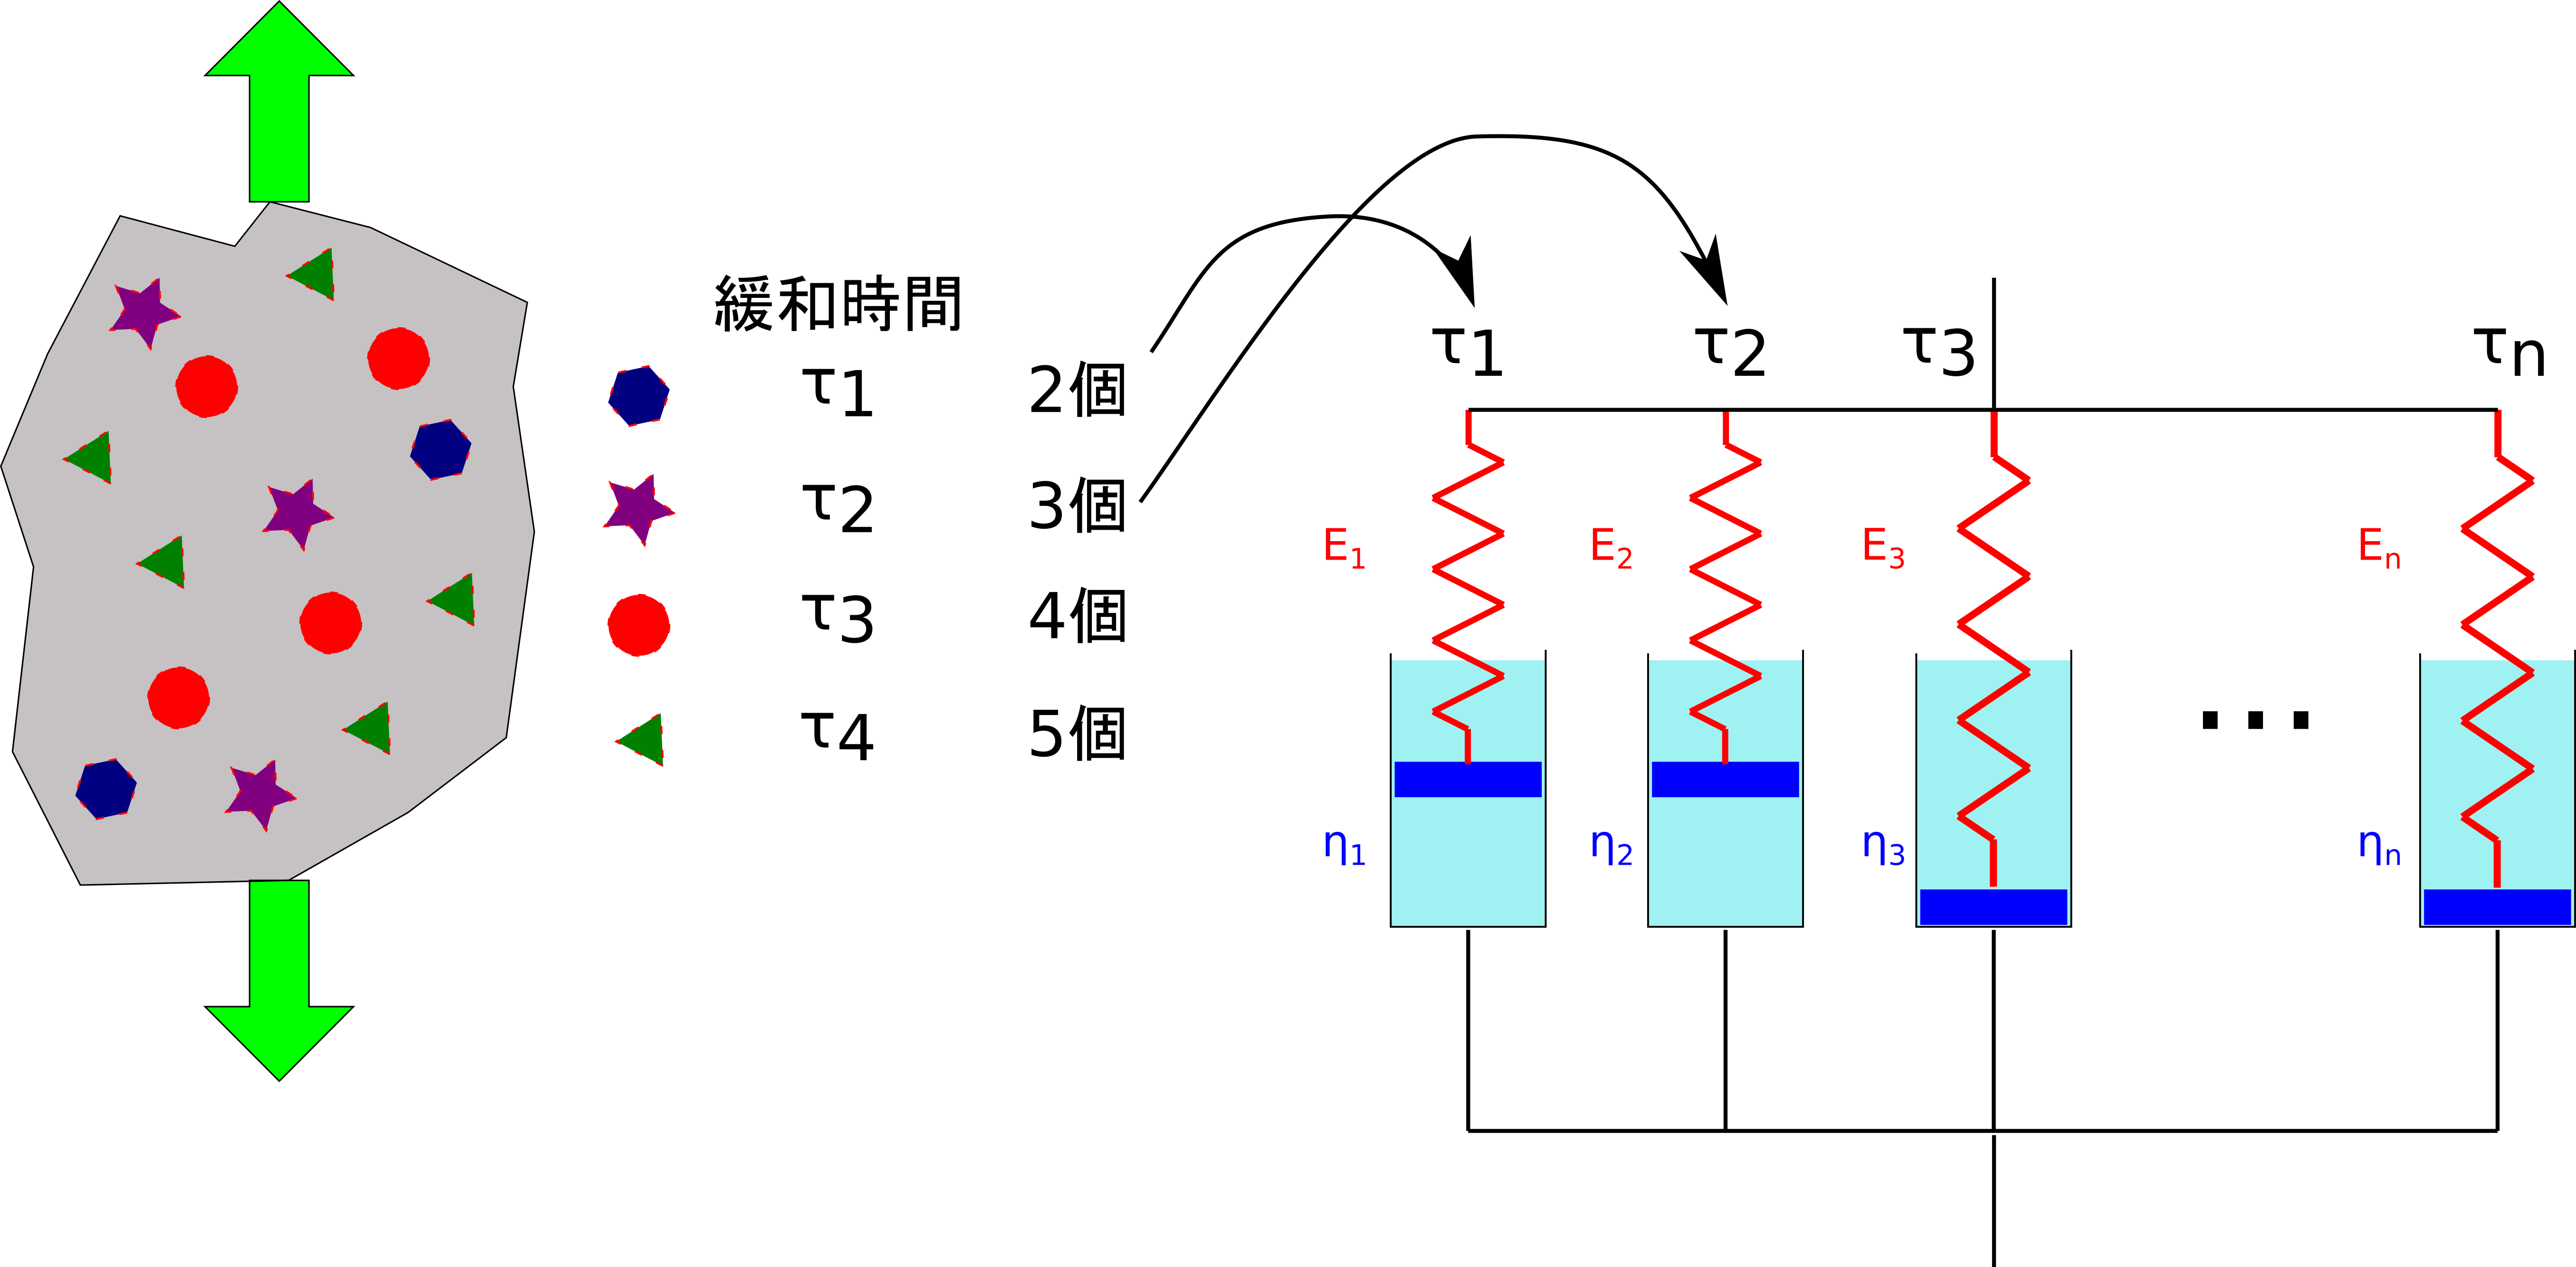
\includegraphics[width=\textwidth]{relux_multi_2.png}
			\end{center}
		\end{minipage}
		\caption{一般化マックスウェルモデル}
		\label{fig:gen_maxwell}
	\end{center}
\end{figure}

このとき、マックスウェルモデル\index{まっくすうぇるもでる@マックスウェルモデル}を並列に連結したのですから、応力\index{おうりょく@応力} $\sigma$ はそれぞれのマックスウェルモデルごとに発生しているものの総和であり、
ひずみ\index{ひずみ@ひずみ} $\varepsilon$ はそれぞれに共通ということになります。

このことを利用して総和の形で書いた表式から誘導することで、結局、
緩和時間\index{かんわじかん@緩和時間}の異なるそれぞれのマックスウェルモデルごとの弾性率\index{だんせいりつ@弾性率}の緩和挙動\index{かんわきょどう@緩和挙動}の総和として書き下すことができるようになります。

\begin{figure}[htb]
	\begin{center}
		\begin{minipage}{0.9\textwidth}
			\begin{itembox}[l]{一般化マックスウェルモデルの数式展開}
				\begin{itemize}
					\item マックスウェルモデルを並列に連結したのだから、
					\begin{itemize}
						\item 応力はそれぞれのものの総和
						\begin{align*}
							\sigma = \sum_{i=1}^n \sigma_i
								= \sum_{i=1}^n \sigma_{0,i}\exp\left(-\dfrac{t}{\tau_i} \right)
						\end{align*}
						\item ひずみ $\varepsilon$ はそれぞれに共通なので、両辺を除して、
						\begin{align*}
							\dfrac{\sigma}{\varepsilon} &= \sum_{i=1}^n \dfrac{\sigma_{0,i}}{\varepsilon}\exp\left(-\dfrac{t}{\tau_i} \right) \\
							\therefore \; E(t) &= \sum_{i=1}^n E_i \exp\left(-\dfrac{t}{\tau_i} \right)
						\end{align*}
					\end{itemize}
					\item 結局、緩和時間の異なるそれぞれのモデルごとの、弾性率\index{だんせいりつ@弾性率}の緩和の総和で表せる。
				\end{itemize}
			\end{itembox}
		\end{minipage}
		\caption{一般化マックスウェルモデルの考え方}
		\label{fig:kanngae_gen_max}
	\end{center}
\end{figure}

\subsubsection{一般化マックスウェルモデルの緩和\index{かんわ@緩和}のイメージ}
この一般化マックスウェルモデル\index{いっぱんかまっくすうぇるもでる@一般化マックスウェルモデル}の緩和現象をイメージ図として表すと、初期状態と変形直後は図 \ref{fig:img_gen_max_0} のように、
すべてのものが同様な変形挙動を受けることになります。

\begin{figure}[htb]
	\begin{center}
		\begin{minipage}{0.45\textwidth}
			\begin{center}
				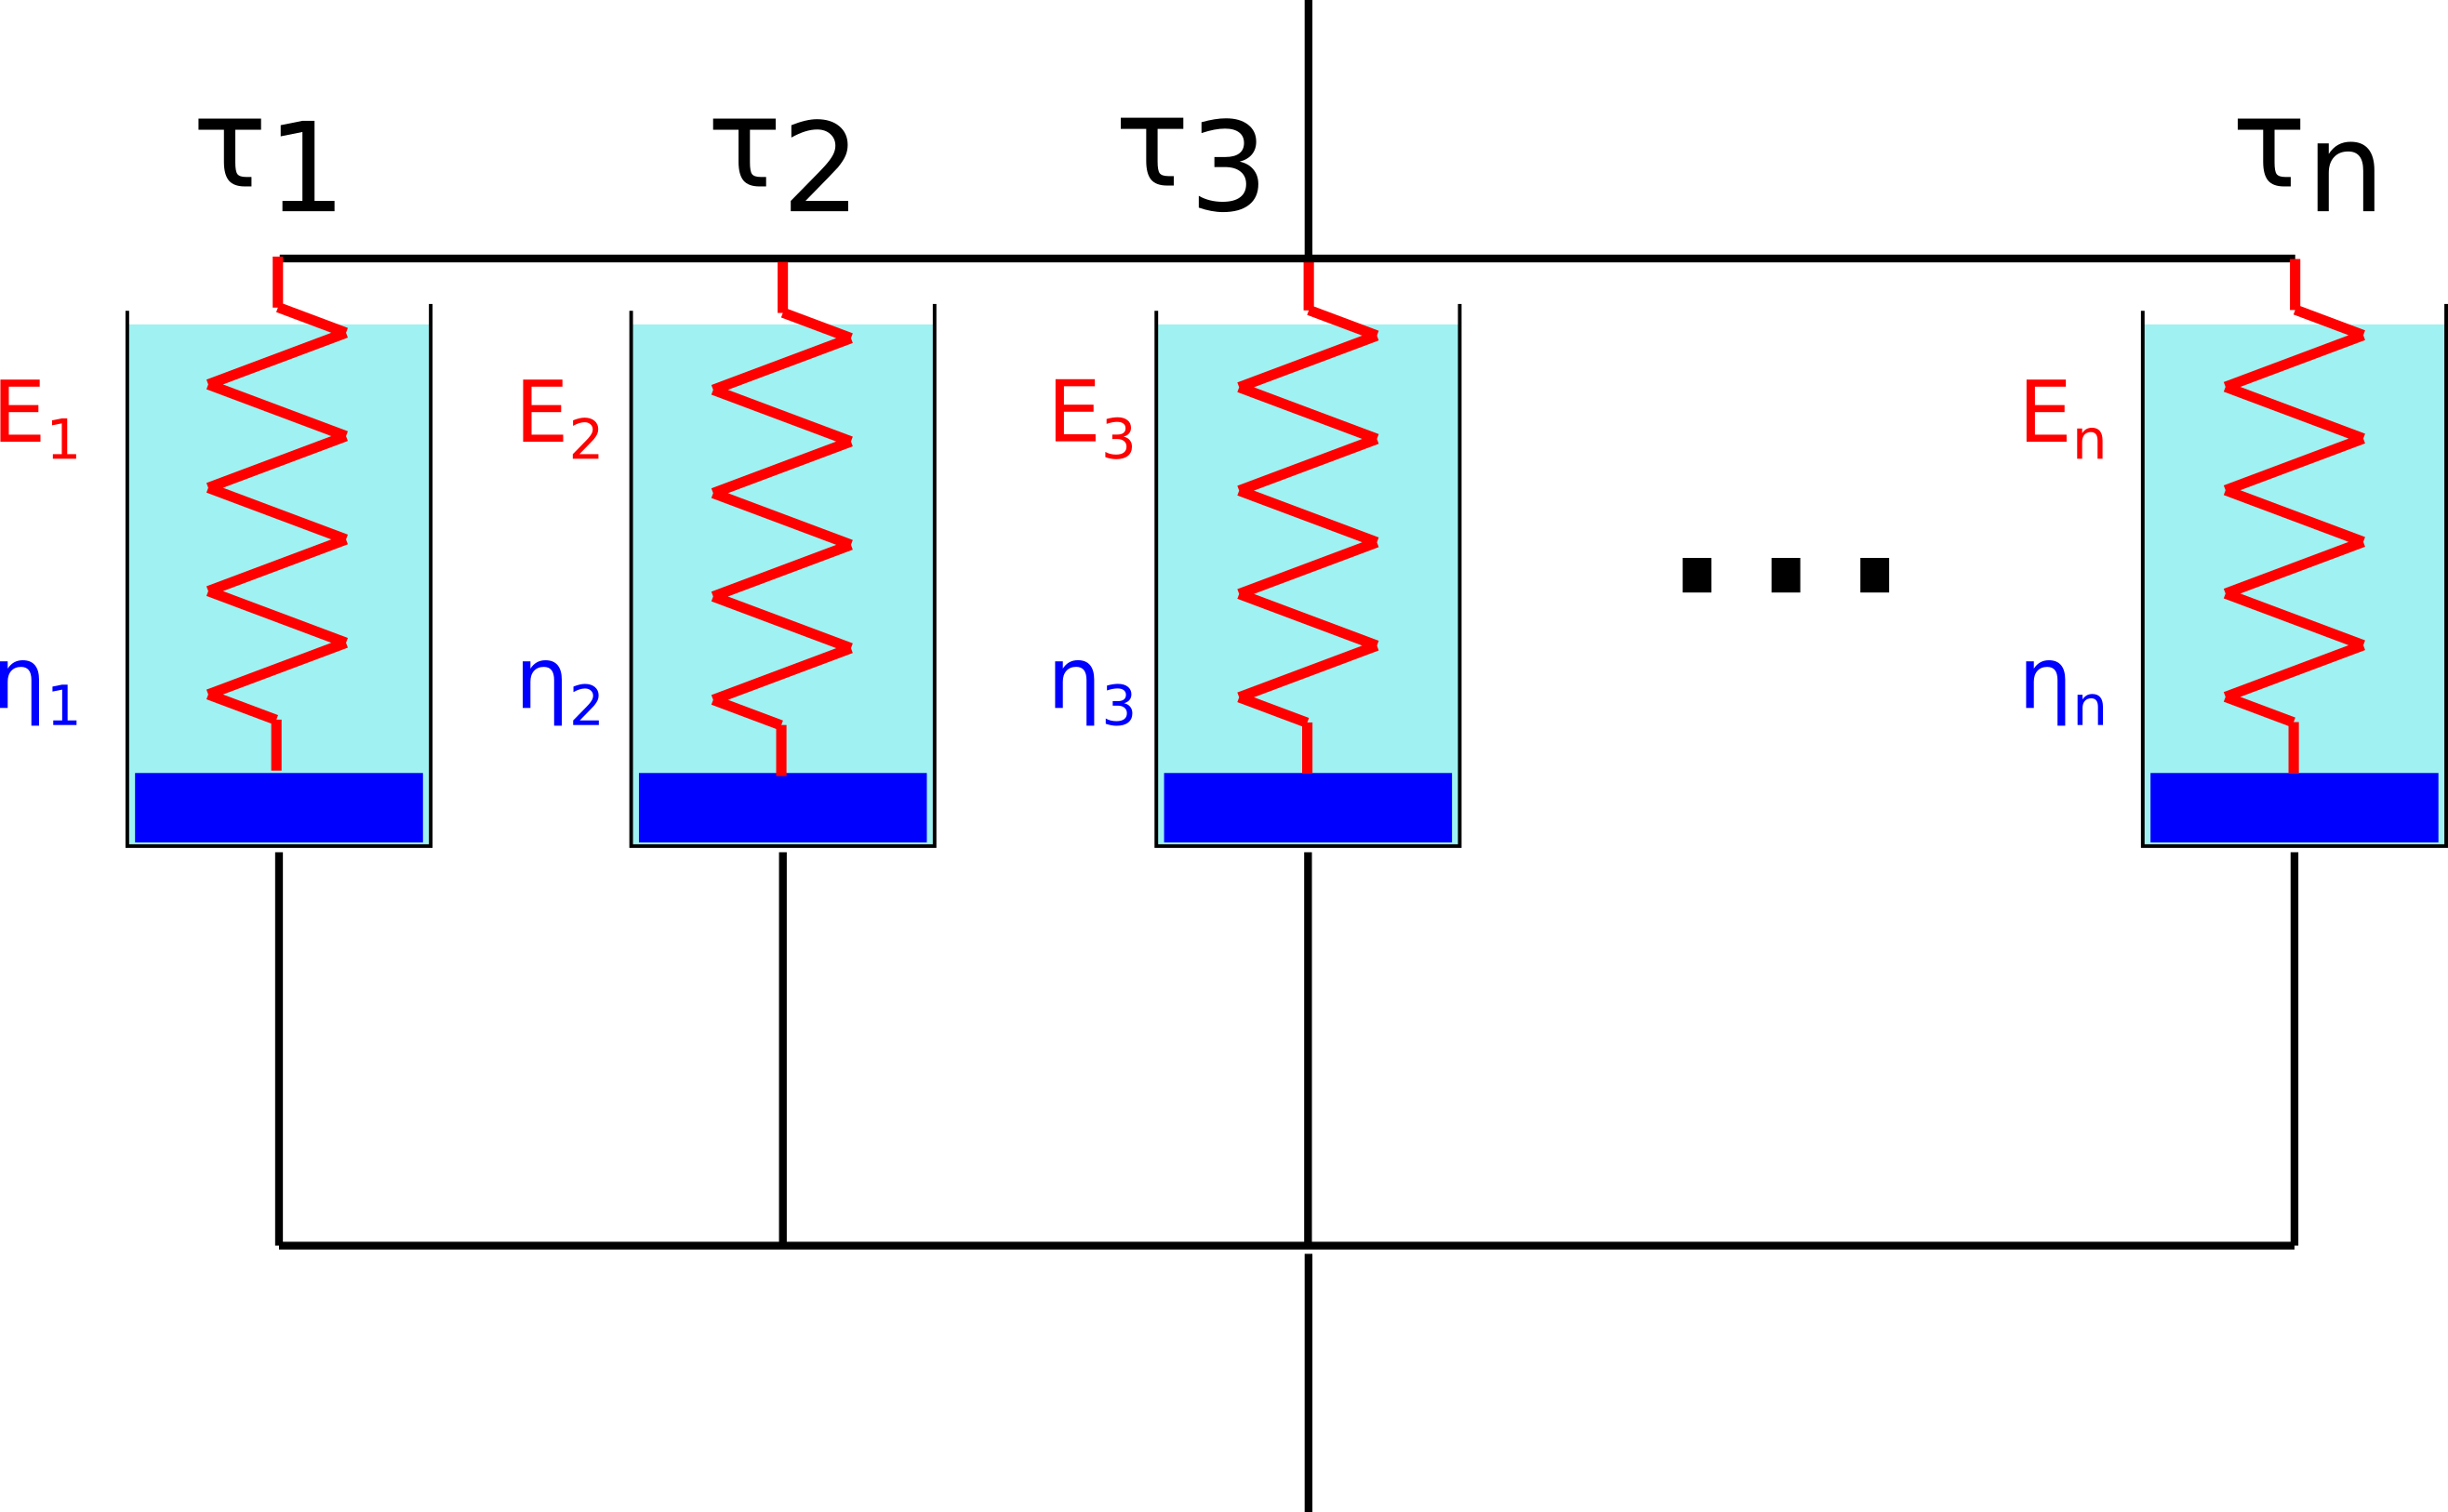
\includegraphics[width=.7\textwidth]{Maxwell_multi_0.png}
			\end{center}
		\end{minipage}
		\begin{minipage}{0.45\textwidth}
			\begin{center}
				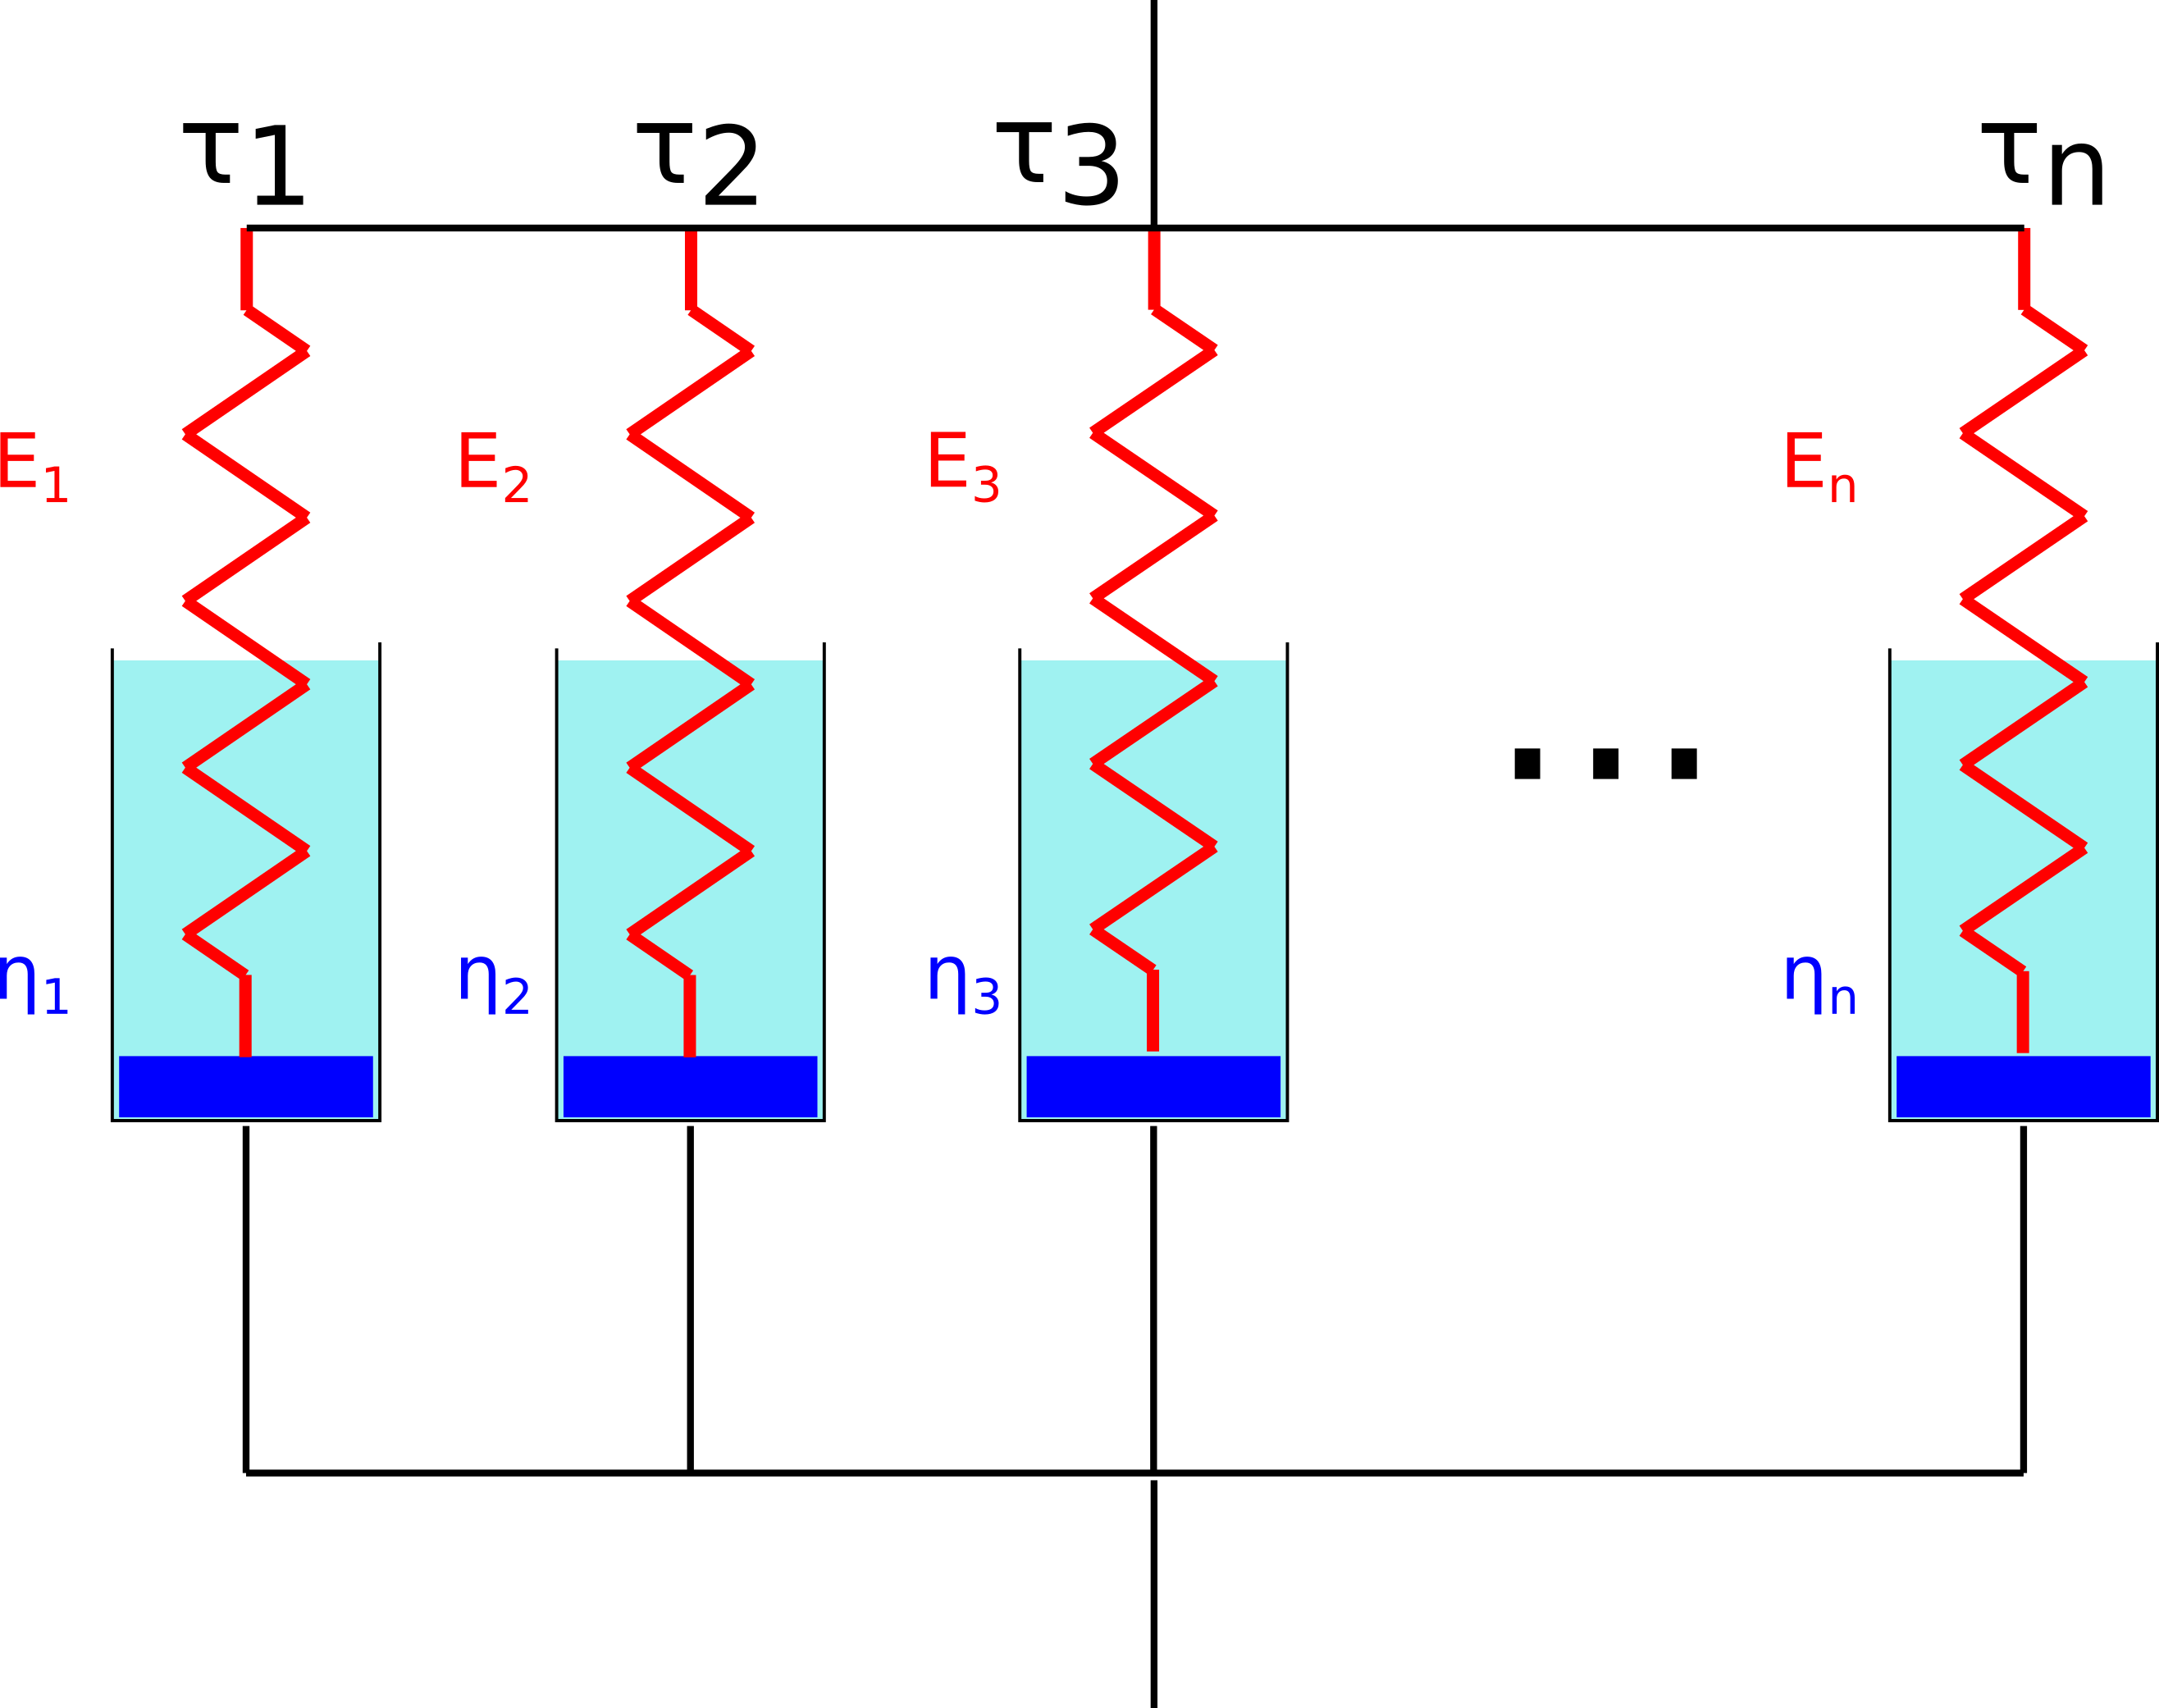
\includegraphics[width=.7\textwidth]{Maxwell_multi_1.png}
			\end{center}
		\end{minipage}
		\caption{緩和のイメージ(初期状態と変形直後)}
		\label{fig:img_gen_max_0}
	\end{center}
\end{figure}

そして、時間の経過に伴って、図 \ref{fig:img_gen_max_1} のように、緩和時間\index{かんわじかん@緩和時間}の短いものから順次緩和が進行していくことになるわけです。

\begin{figure}[htb]
	\begin{center}
		\begin{minipage}{0.45\textwidth}
			\begin{center}
				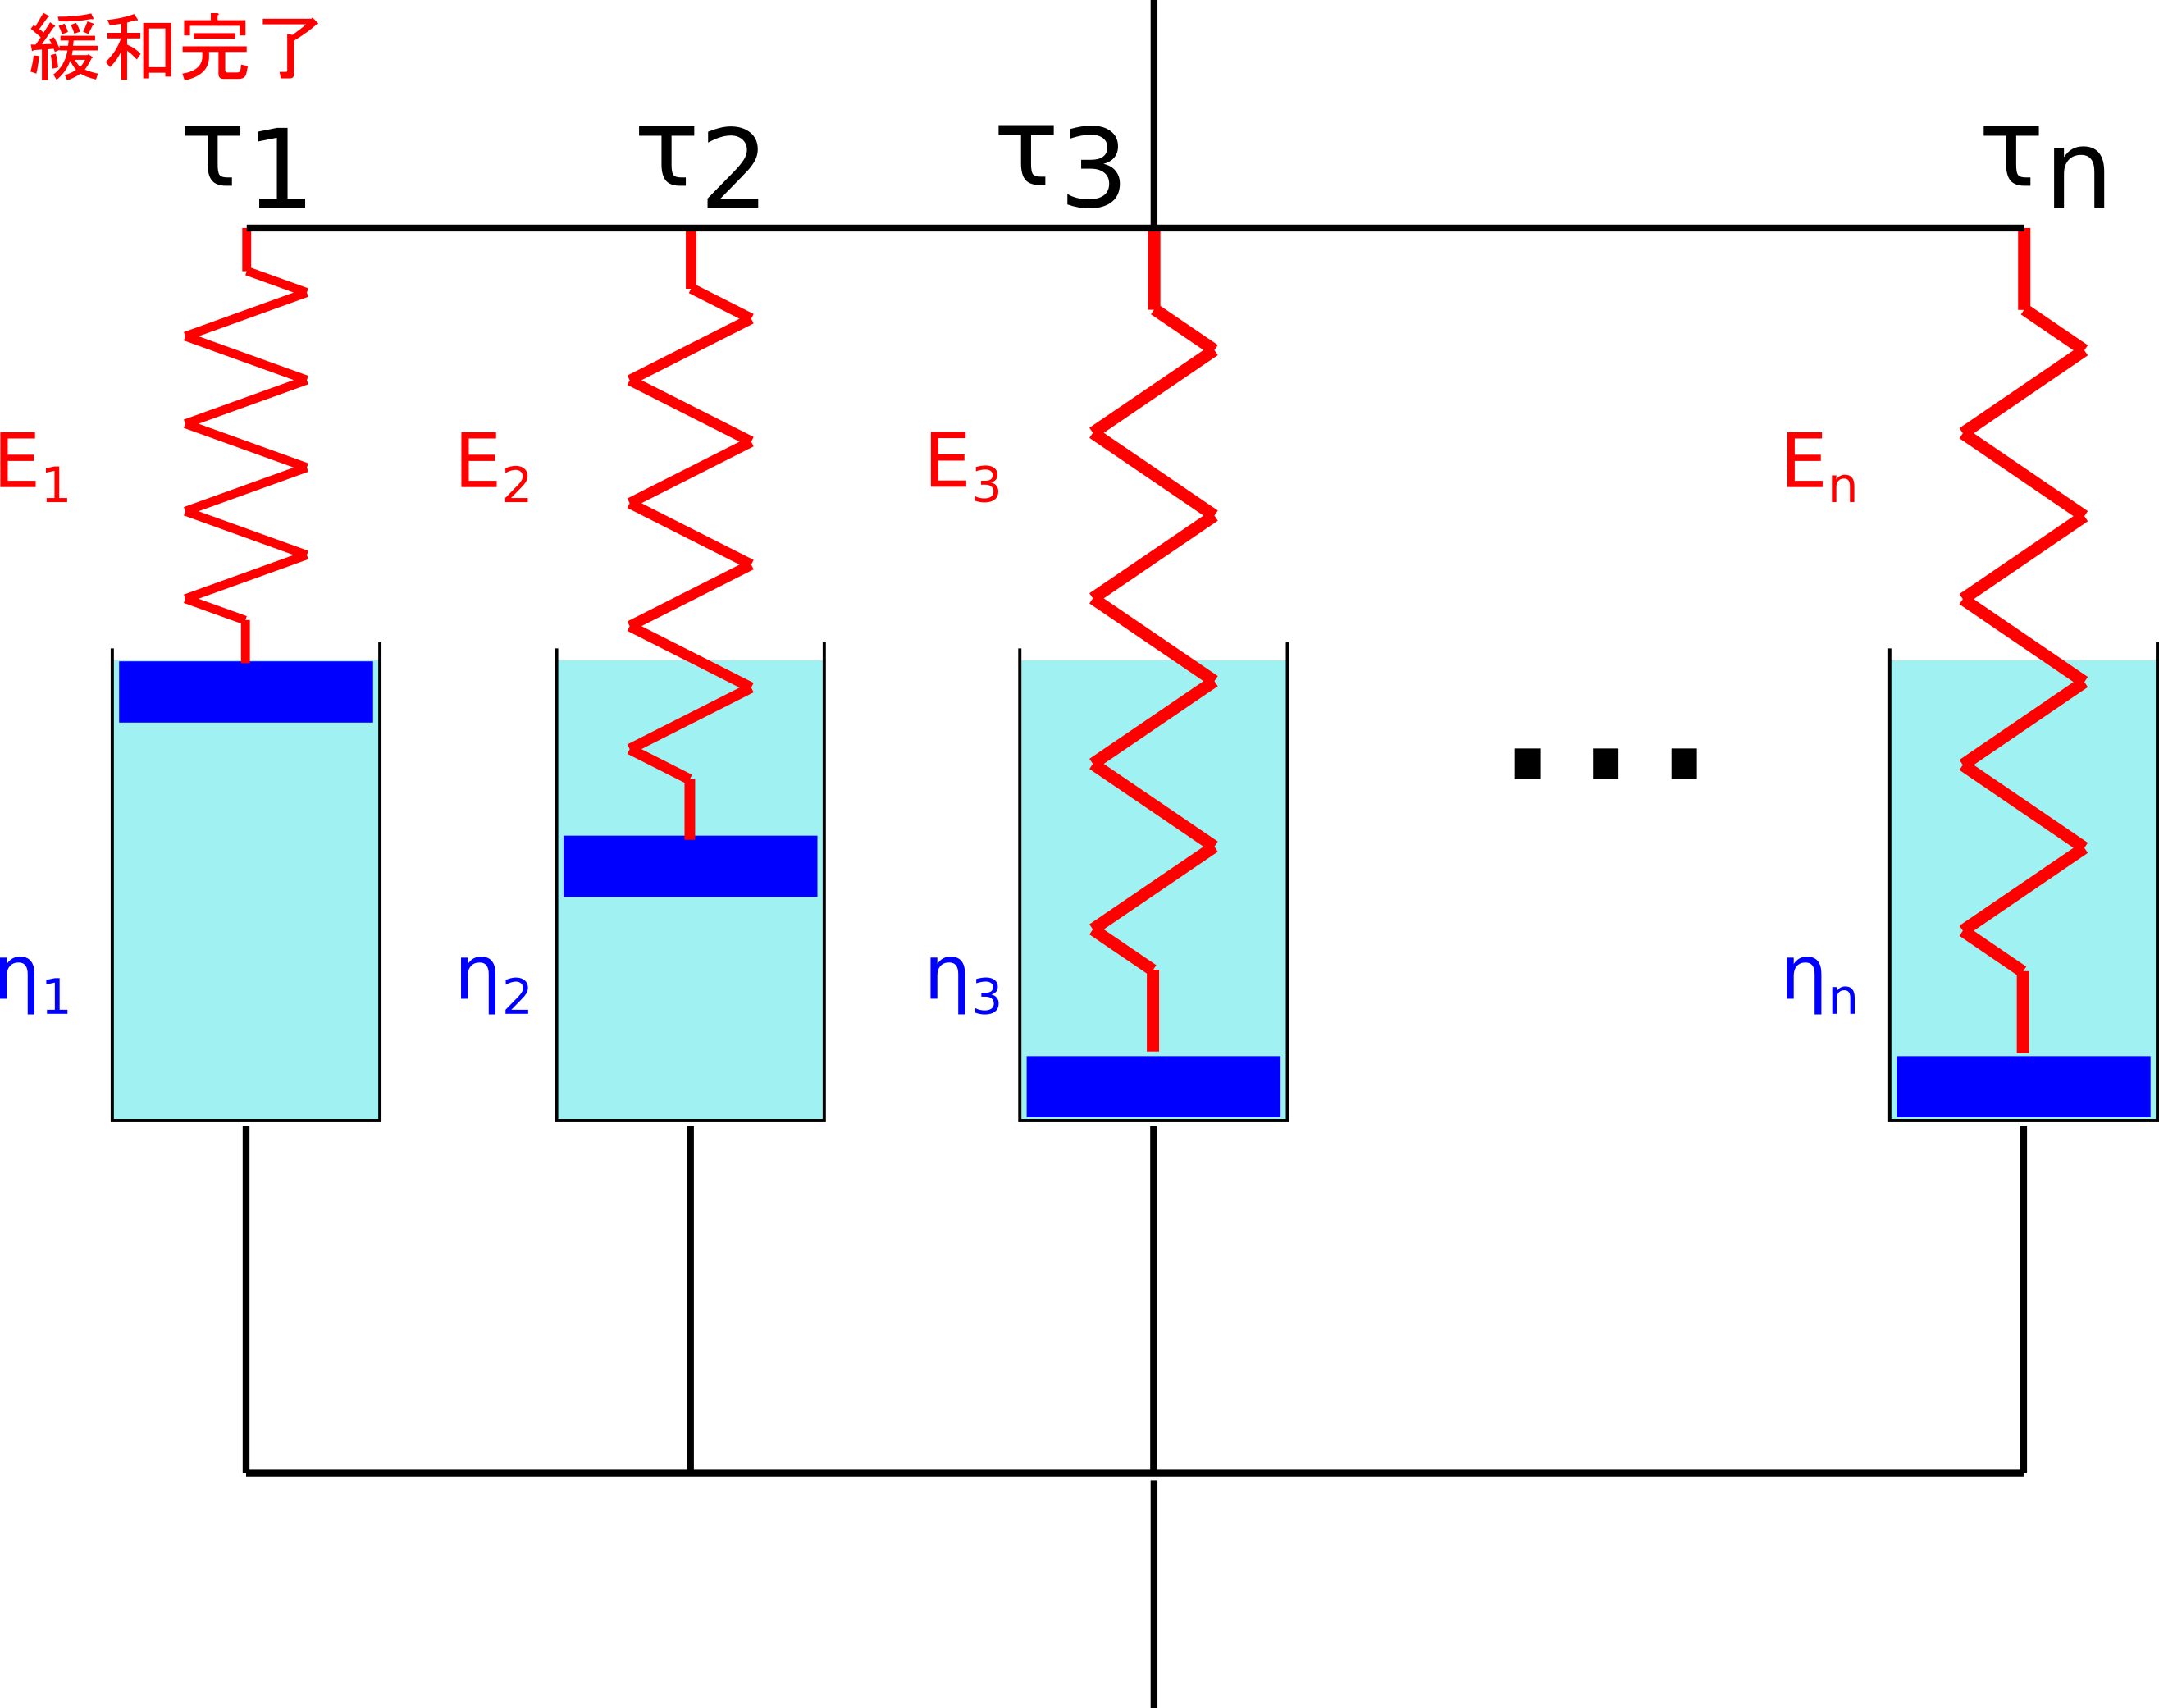
\includegraphics[width=.7\textwidth]{Maxwell_multi_2.png}
			\end{center}
		\end{minipage}
		\begin{minipage}{0.45\textwidth}
			\begin{center}
				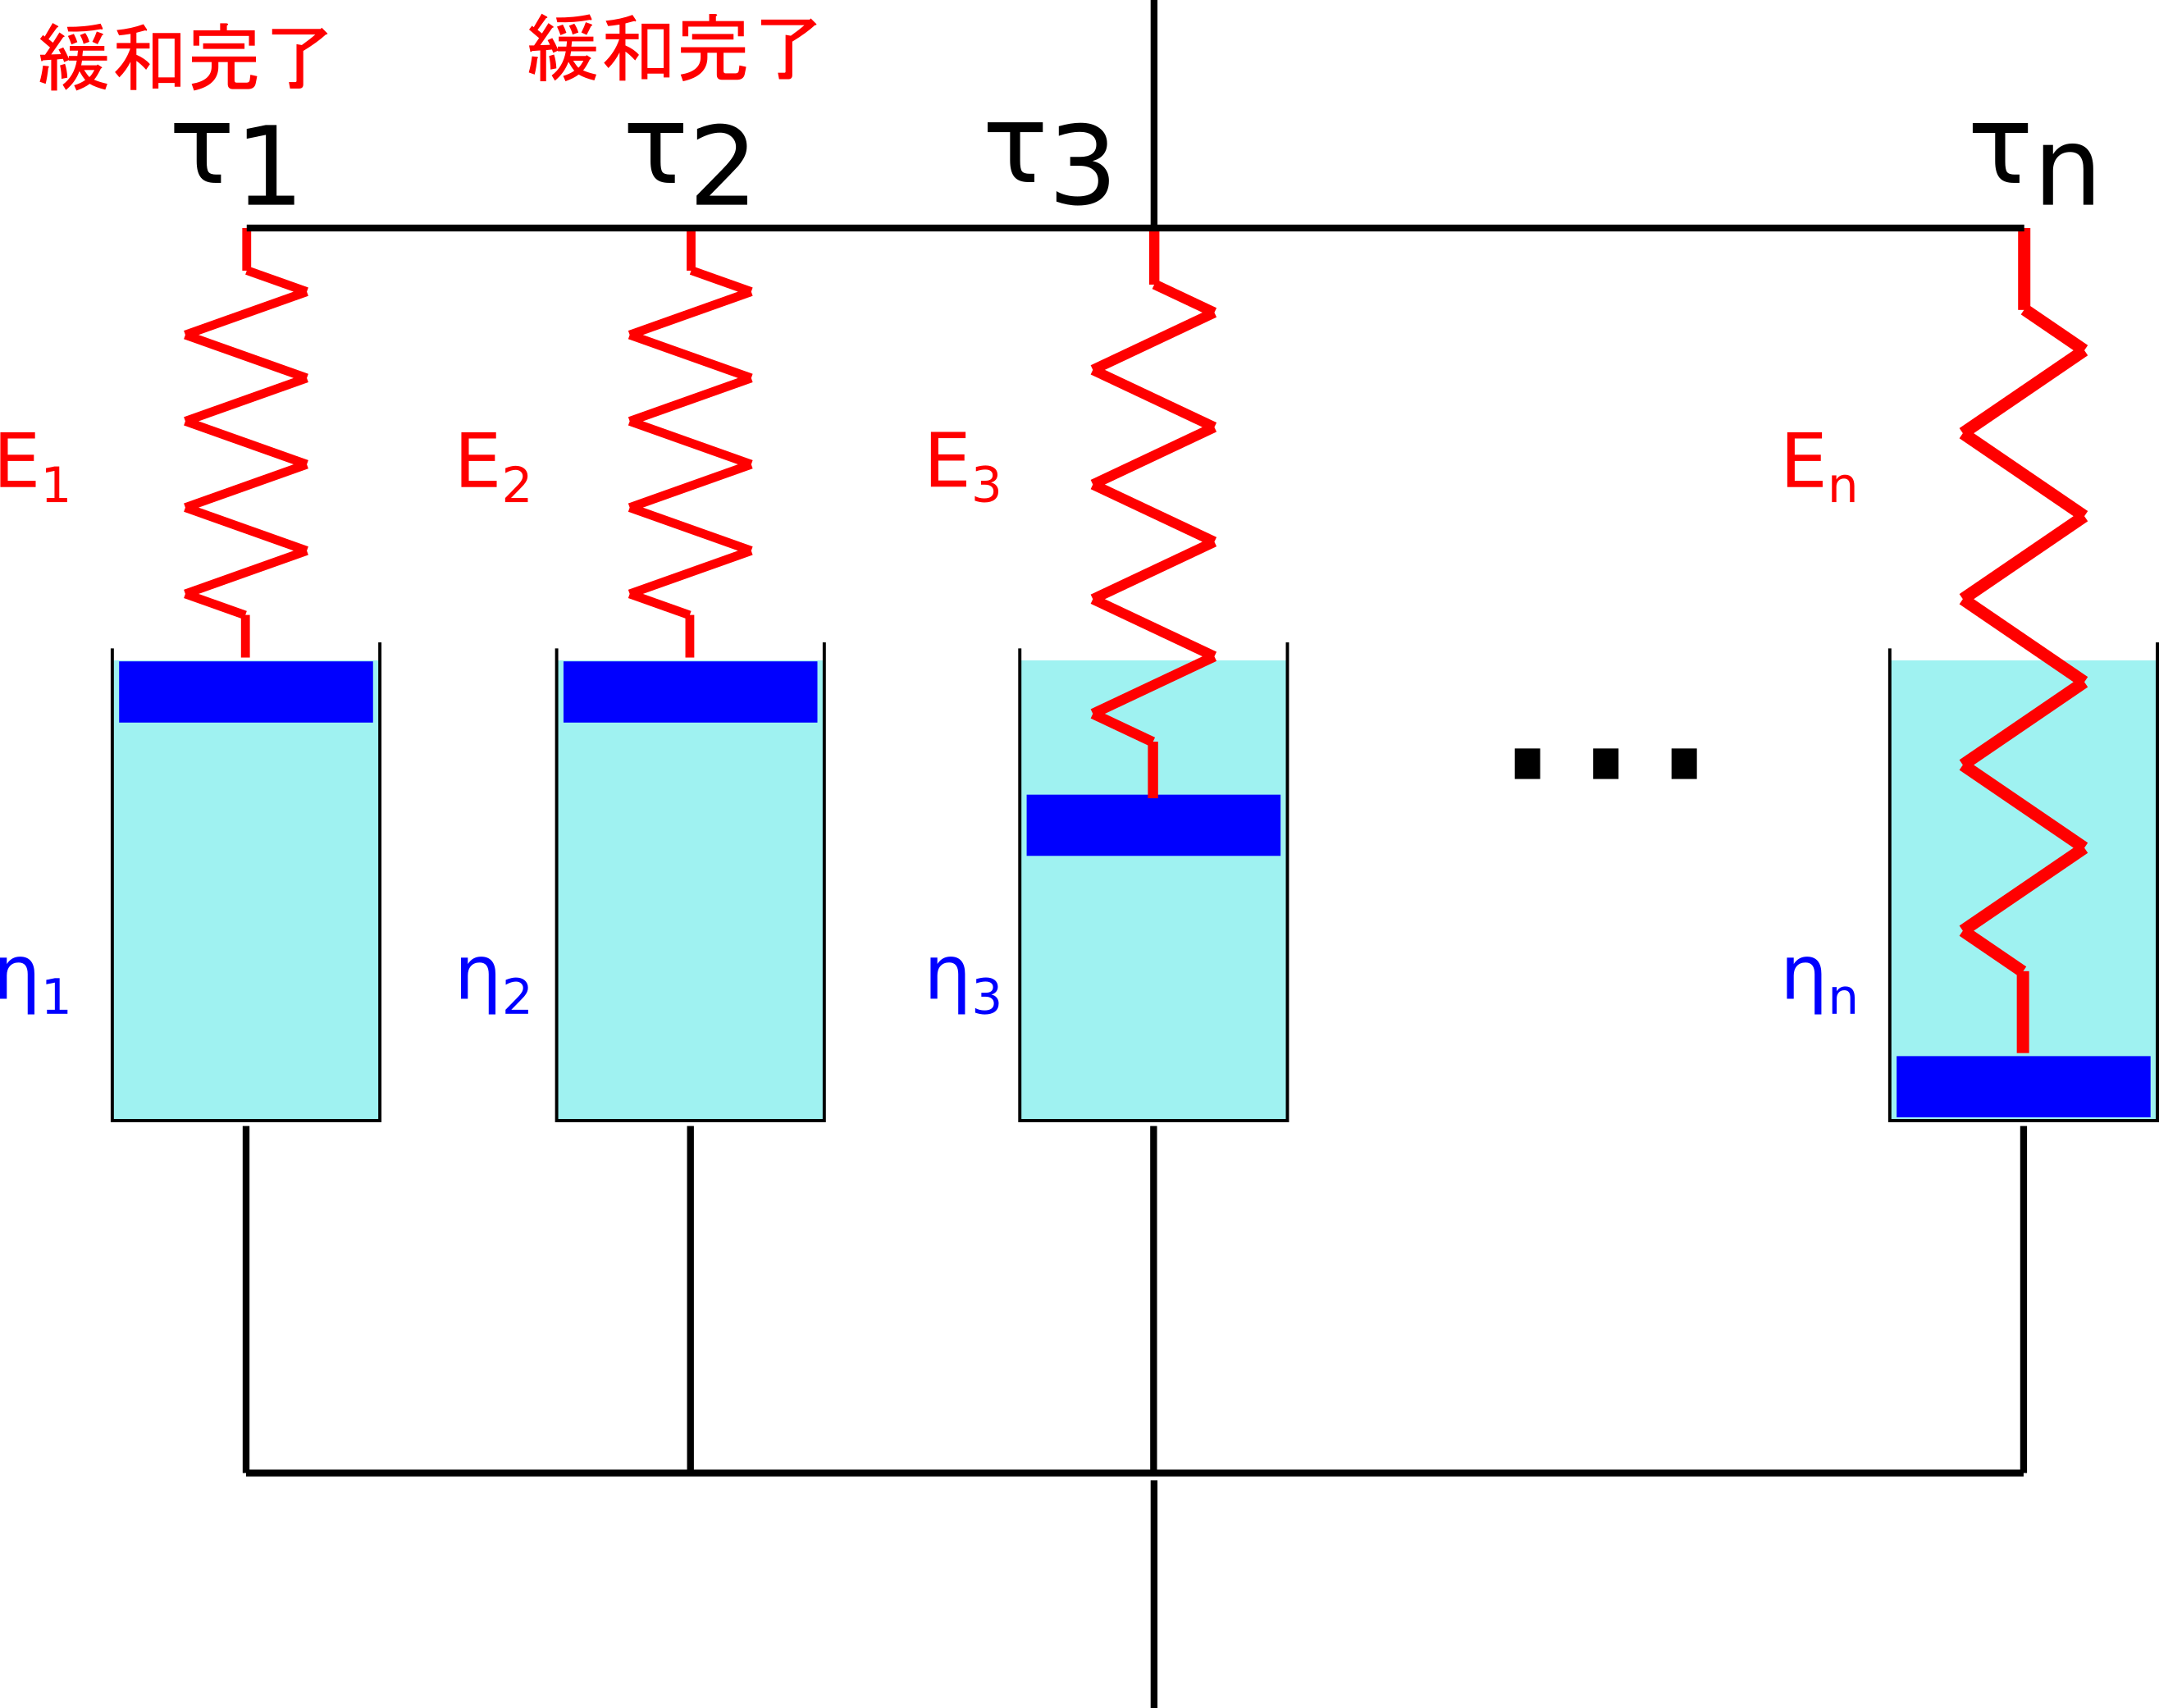
\includegraphics[width=.7\textwidth]{Maxwell_multi_3.png}
			\end{center}
		\end{minipage}
		\caption{緩和のイメージ(任意の時間経過)}
		\label{fig:img_gen_max_1}
	\end{center}
\end{figure}

\subsubsection{緩和\index{かんわ@緩和}のプロット}
	\begin{center}
		\begin{minipage}{0.9\textwidth}
			\begin{itembox}[l]{一般化マックスウェルモデルの緩和挙動\index{かんわきょどう@緩和挙動}}
				\begin{itemize}
					\item 個々のマックスウェルモデルの緩和挙動の和の形で記述され、
					\item 仮に緩和強度が同一とすると、右図のように単純な和となり、
					\item 時間の経過に従って、緩和時間の短いものから順次緩和していく。
				\end{itemize}
			\end{itembox}
		\end{minipage}
	\end{center}

図 \ref{fig:plot_gen_max} に、その緩和挙動\index{かんわきょどう@緩和挙動}をプロットしたイメージを示しました。
\begin{figure}[htb]
	\begin{center}
		\begin{minipage}{0.45\textwidth}
			\begin{center}
				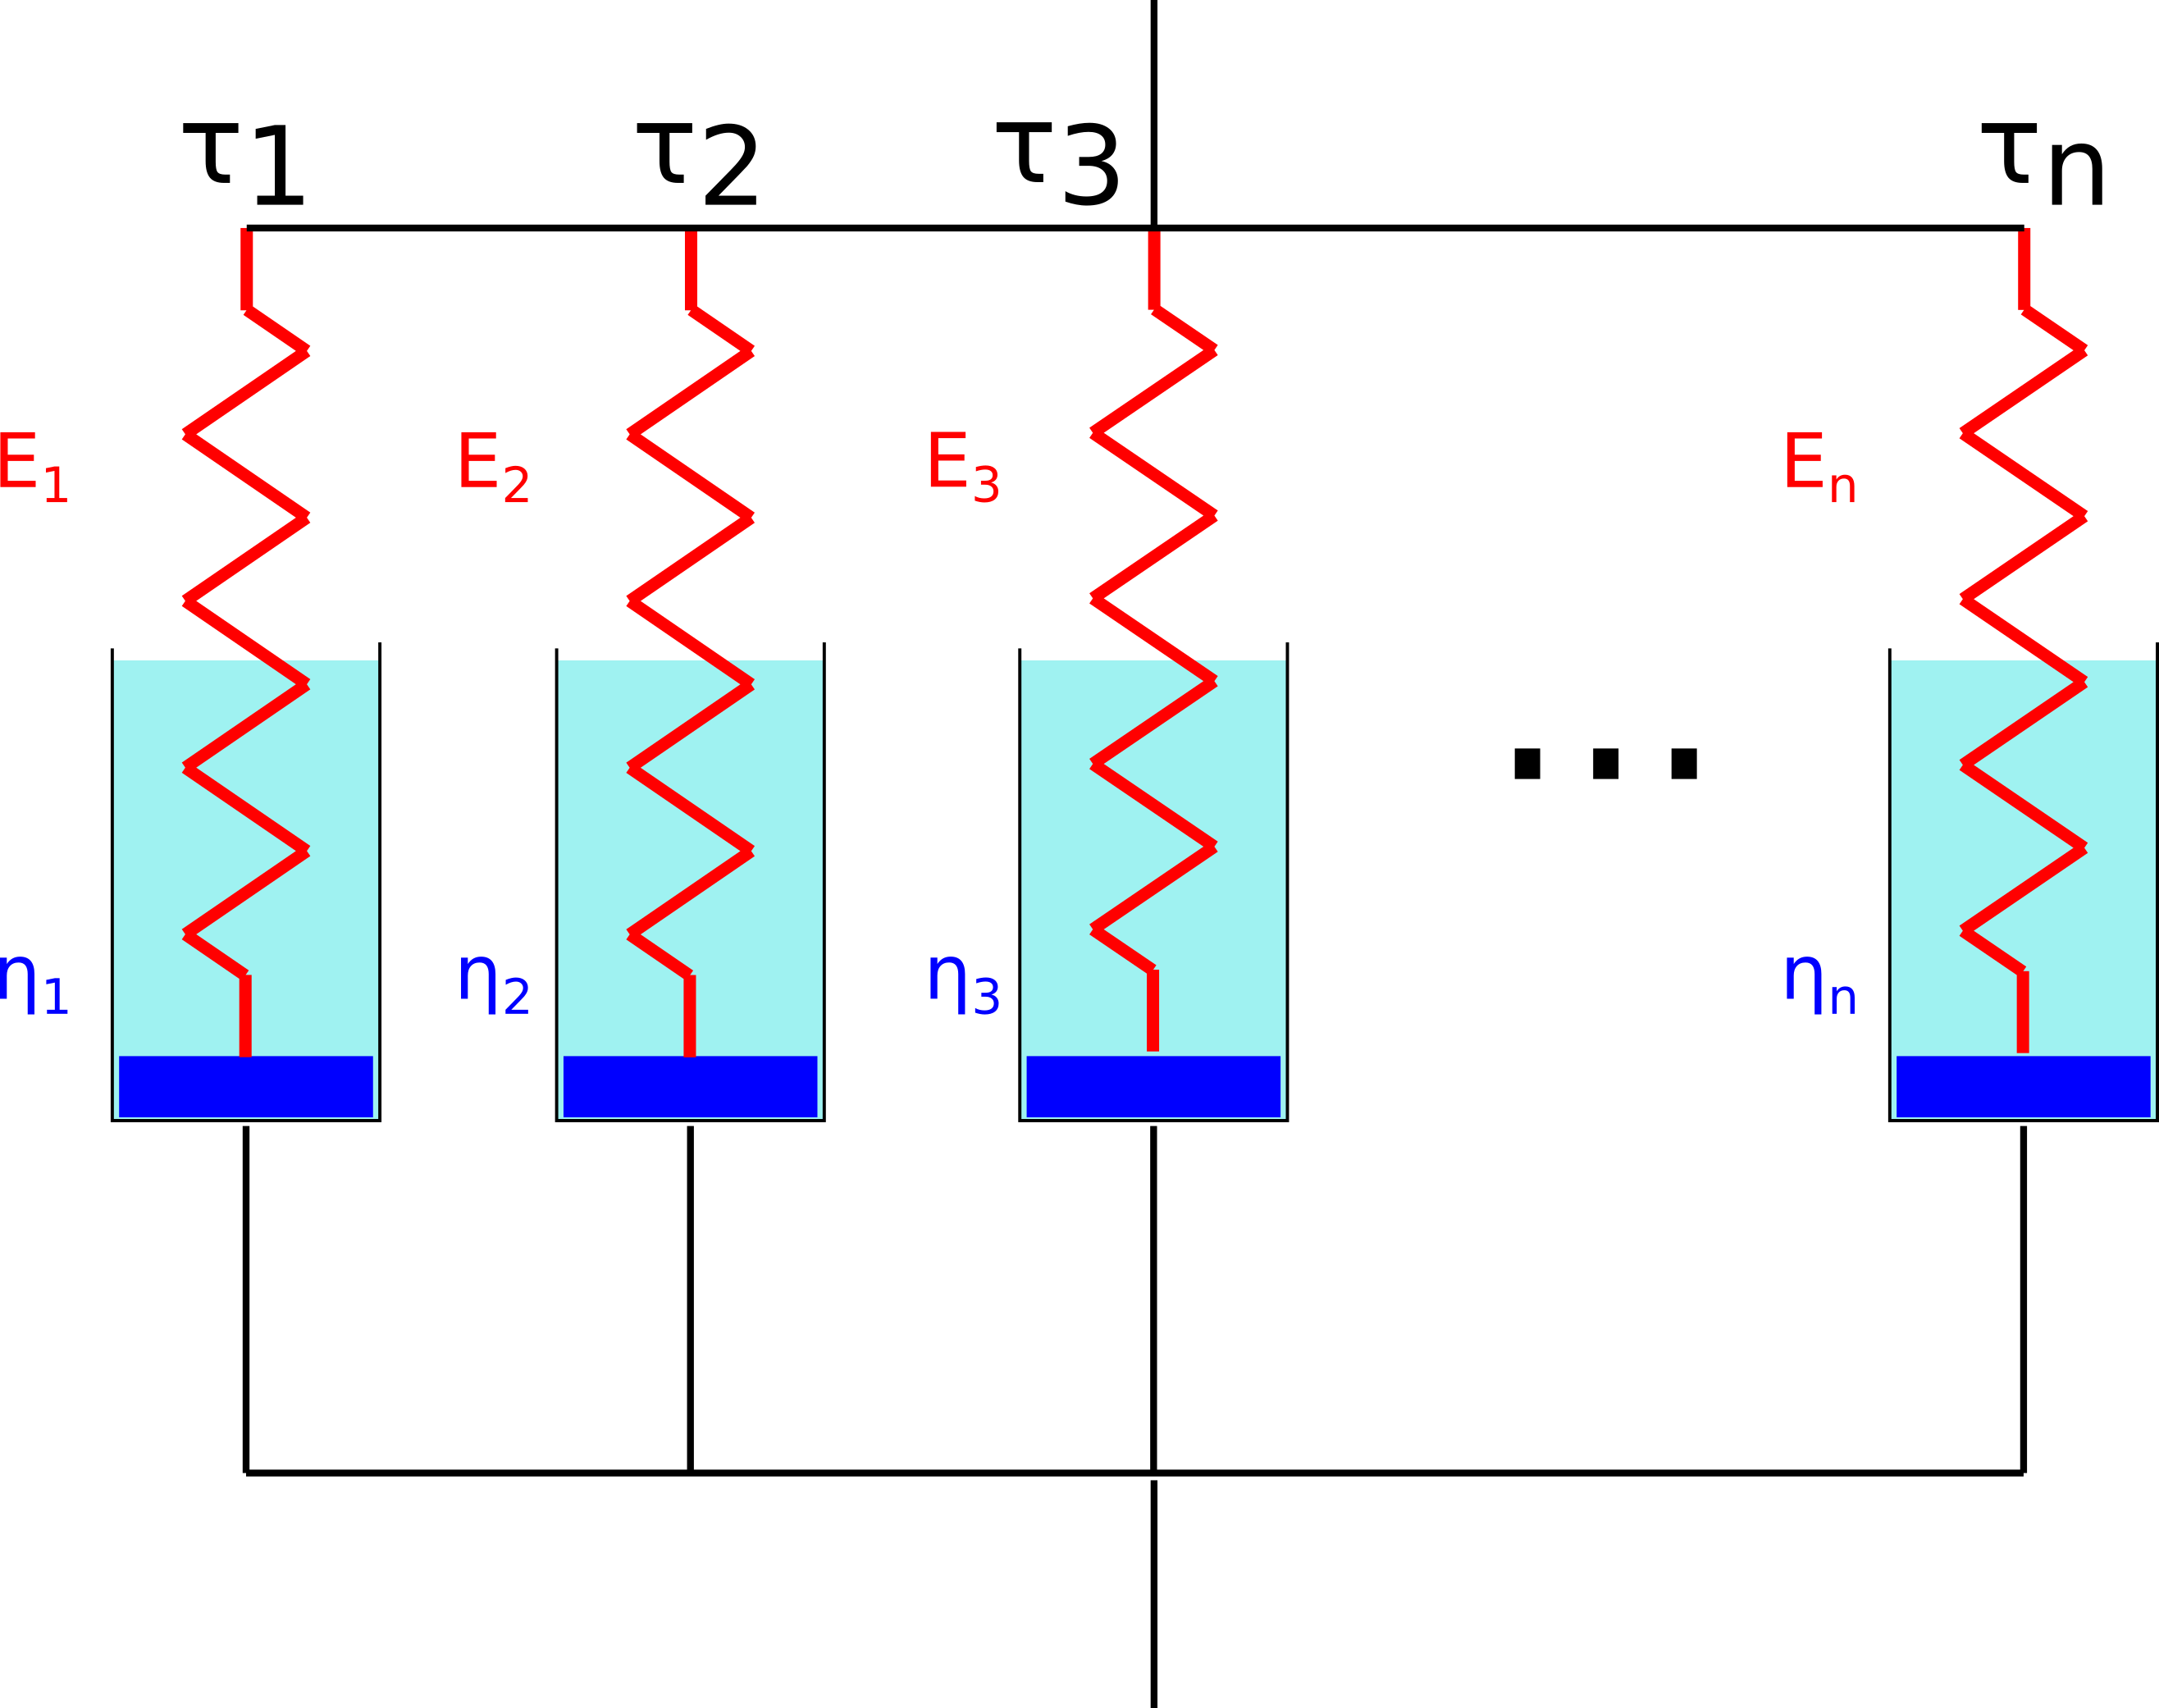
\includegraphics[width=\textwidth]{Maxwell_multi_1.png}
			\end{center}
		\end{minipage}
		\begin{minipage}{0.45\textwidth}
			\begin{center}
				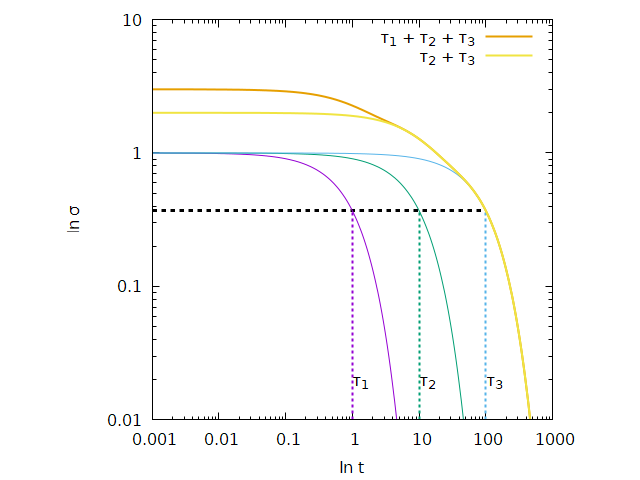
\includegraphics[width=\textwidth]{relux_8.png}
			\end{center}
		\end{minipage}
		\caption{緩和のプロット}
		\label{fig:plot_gen_max}
	\end{center}
\end{figure}



\subsection{固体と液体の判断}
最後に、固体\index{こたい@固体}と液体\index{えきたい@液体}とを判断する一つの基準について考えてみましょう。

\subsubsection{応力緩和での固体と液体}
応力緩和\index{おうりょくかんわ@応力緩和}を観察するということは、ステップひずみを物質に付与してから長時間領域での緩和挙動を見ることになります。
このとき、図 \ref{fig:kotaitoekitai} に示したように、任意の観察時間\index{かんさつじかん@観察時間}において緩和しきれない弾性率(応力\index{おうりょく@応力})成分が残存している場合、
その観察においては固体\index{こたい@固体}として振る舞っているということになるわけです。
一方、その観察時間\index{かんさつじかん@観察時間}において、応力\index{おうりょく@応力}が残存しないのであれば、それは液体\index{えきたい@液体}として取り扱うことができます。

\begin{figure}[htb]
	\begin{center}
		\begin{minipage}{0.45\textwidth}
			\begin{itembox}[l]{粘弾性体の特徴}
				\begin{itemize}
					\item ステップひずみの長時間の緩和で、
					\item $E \rightarrow 0$\\
					流動する粘弾性液体
					\item 固体は緩和しない成分が残存
				\end{itemize}
			\end{itembox}
		\end{minipage}
		\begin{minipage}{0.45\textwidth}
			\begin{center}
			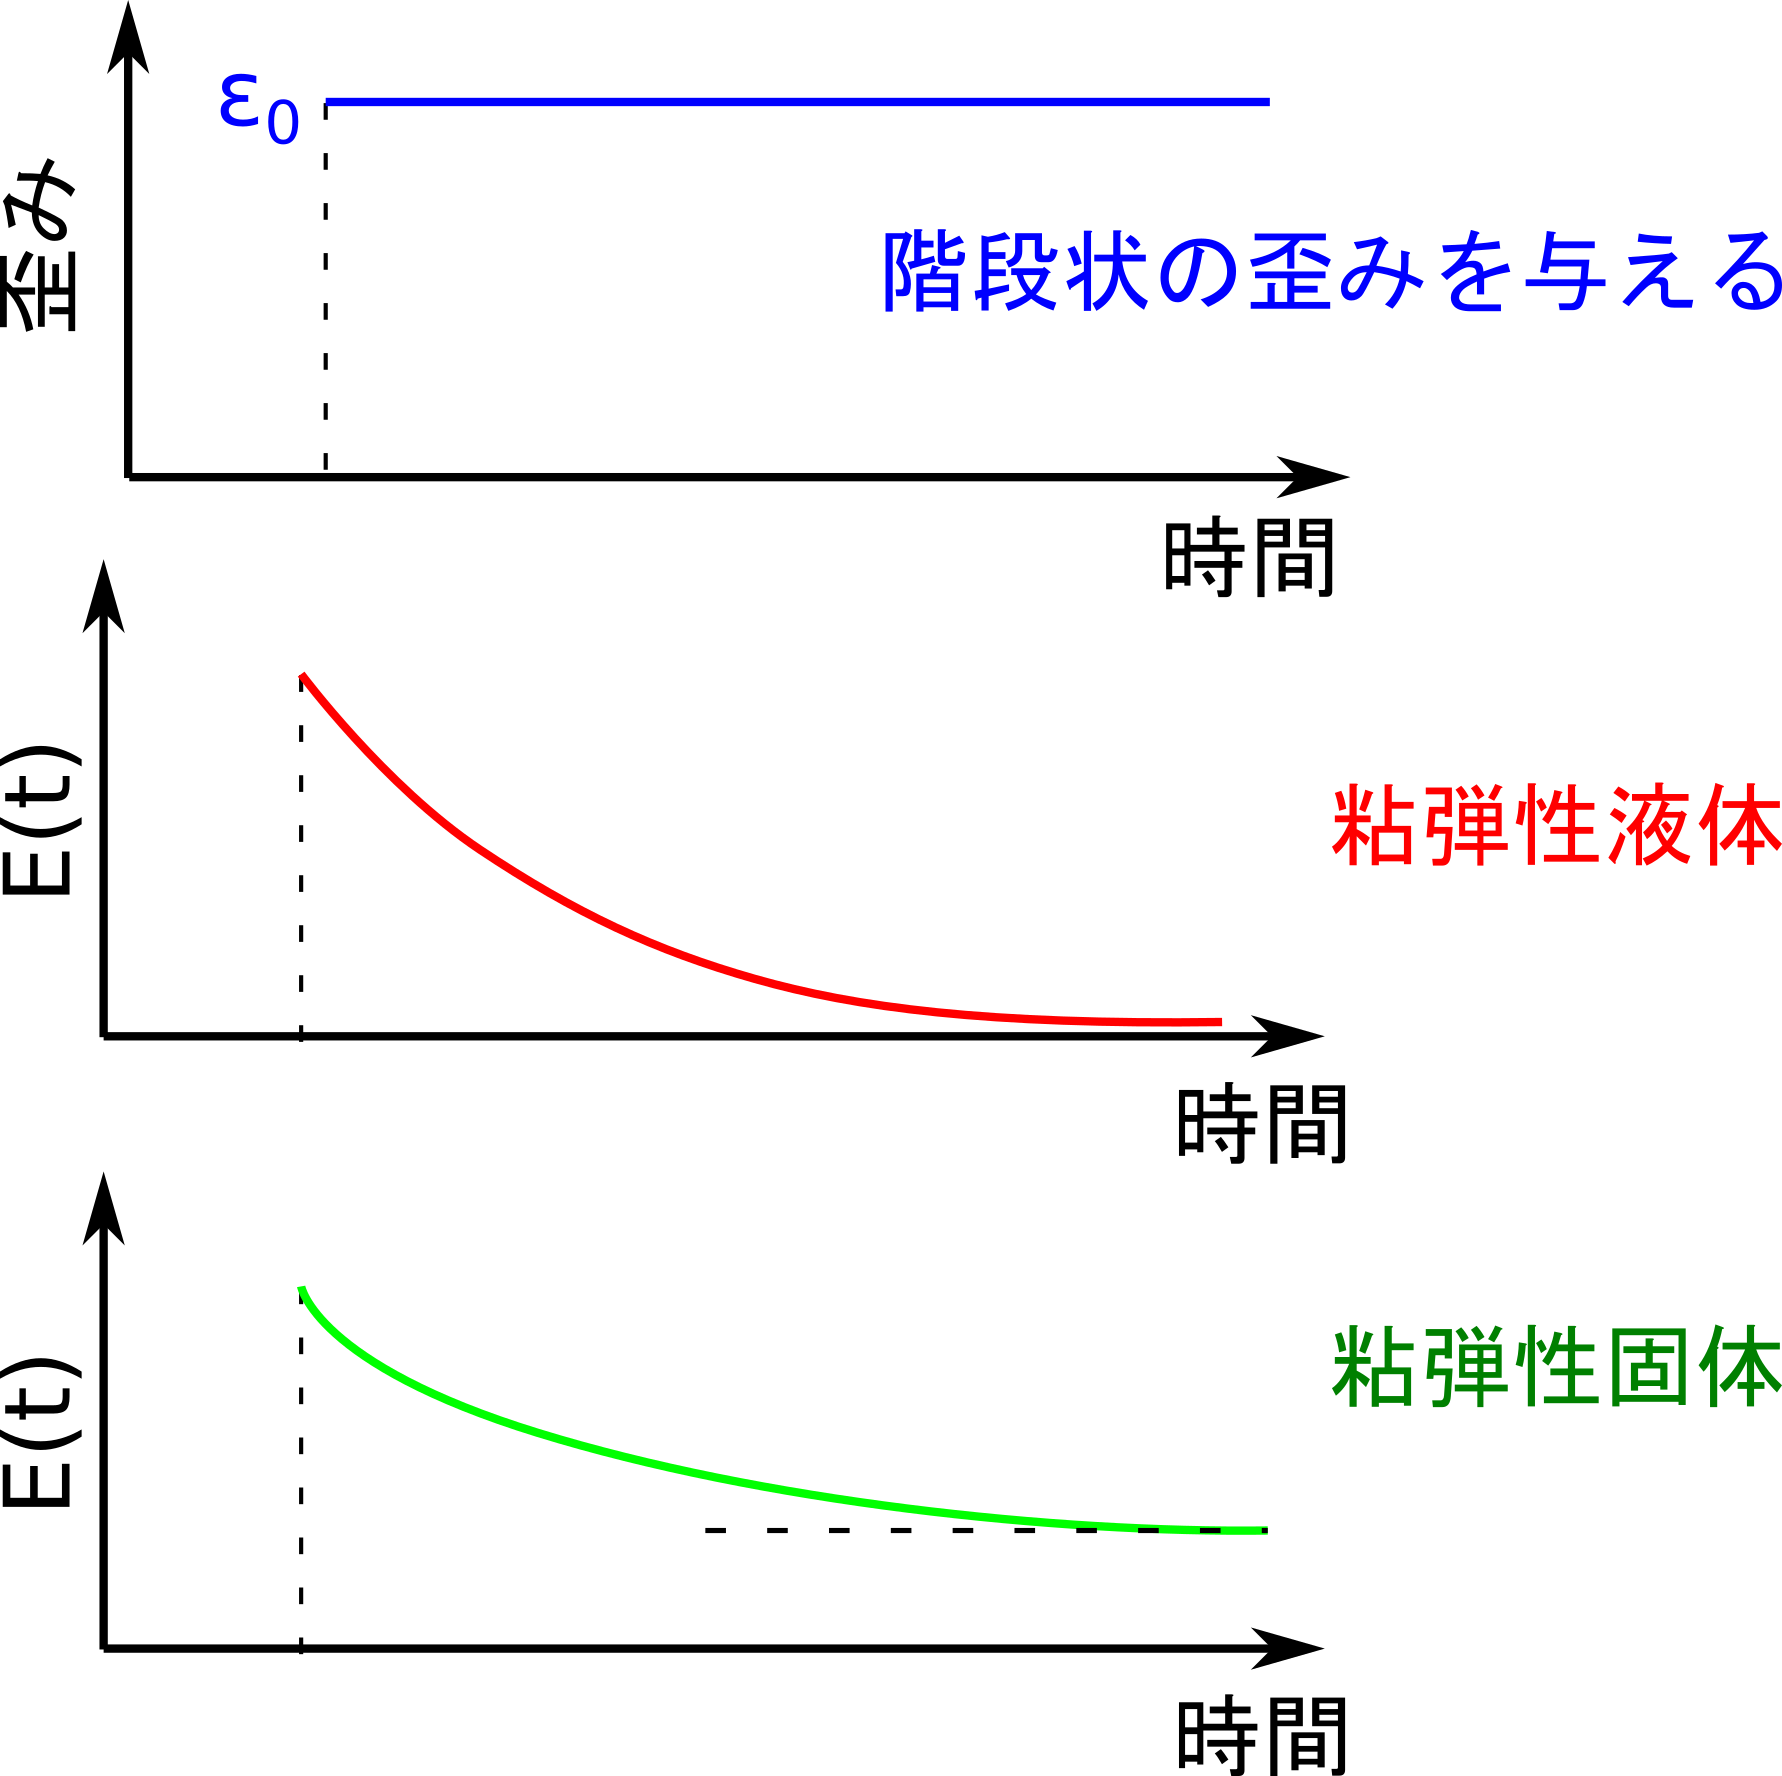
\includegraphics[width=.8\textwidth]{stress_solid_liquid.png}
			\end{center}
		\end{minipage}
		\caption{応力緩和で見た固体と液体}
		\label{fig:kotaitoekitai}
	\end{center}
\end{figure}

\subsubsection{デボラ数}

物質の持つ緩和時間と観察時間\index{かんさつじかん@観察時間}との関係は、デボラ数\index{でぼら@デボラ数} $D_e$ と呼ばれる無次元量で直感的に理解することができます。
\begin{align*}
	D_e = \dfrac{\text{緩和時間}}{\text{観察時間}}
\end{align*}

結局、固体\index{こたい@固体}と液体\index{えきたい@液体}の区別は相対的なものであり、レオロジー的には以下のように定義されます。

	\begin{center}
		\begin{minipage}{0.9\textwidth}
			\begin{center}
				\begin{itembox}[l]{デボラ数での区別}
					\begin{itemize}
						\item $D_e << 1$ ならば、緩和時間が小さいので流動し、液体。
						\item $D_e >> 1$ ならば、観測時間において物質は緩和しないので、固体。
					\end{itemize}
				\end{itembox}
			\end{center}
		\end{minipage}
	\end{center}

\section*{この章のまとめ}
この章では、粘性と弾性についての基本的なモデルであるフック固体\index{ふっくこたい@フック固体}とニュートン流体\index{にゅーとんりゅうたい@ニュートン流体}をベースとして、
その組み合わせとして時間に伴い変化していく複雑な現象である粘弾性へとつなげていく議論を行いました。
\begin{boxnote}
    \begin{itemize}
        \item 粘性と弾性についての再確認を行い、
            \begin{itemize}
                \item 固体と液体の応答について振り返ったうえで、
                \item その組み合わせとしての粘弾性を議論しました。
            \end{itemize} 
        \item 粘弾性のモデル化は、
            \begin{itemize}
                \item 粘弾性の単純なモデルであるマックスウェルモデルにより、
                \item 応力緩和と緩和時間を考えました。
            \end{itemize} 
        \item 少しだけ実事象に近づけるために、
            \begin{itemize}
                \item 複数の緩和時間を一般化マックスウェルモデルを用いて議論することで、
                \item 粘弾性的に固体と液体の違いが、応力緩和で理解できることを示しました。
            \end{itemize}
    \end{itemize}
\end{boxnote}

\newpage

\begin{longartdeco}
	\begin{center}
	\emph{コラム:応力とストレス}	
	\end{center}

	レオロジーを学ぶ人達は、かなり最初の段階で説明される連続体力学という形で、変形と応力について教えられます。
	あの「棒を引っ張って伸ばして、その内部に応力という逆向きの2つの矢印を書いた」絵のことです。
	そこでは、応力とは、「外部から変形を付与」したときに、その刺激に「応じて(物体の内部で)生じる力」というように表現されます。
	
	応力という言葉には、「力」という文字が入っているので、応力と力が同じものだと考えてしまいがちなんですが、この勘違いが、結構、応力の理解を難しくしているのかもしれません。
	
	普段の日常会話でストレスと言えば、「心理的ストレス」を指します。
	この文脈でのストレスという言葉は、自分たちにとって望ましくない状態を引き起こす「要因」を指すこともあれば、それによって引き起こされた望ましくない「状態」を指すこともあり、「原因と結果の2つの意味合い」で使用されています。
	これが、また、混乱を招いているのかもしれません。
	
	この心理的ストレスという考え方は、Seyle というカナダの生理学者が定義したものとされています。
	彼の定義において、ストレスは「生体に影響を及ぼす外的刺激によって引き起こされる生体が示す反応」とされています。
	そして、ストレスの原因となる刺激を「ストレッサー」と呼び、心理面、身体面、行動面の反応として現れる生体の反応を「ストレス反応」と呼びます。
	彼が、心理的状態に持ってきたこの考え方は、オリジナルとなる力学的作用を心理に焼き直したものであり、きれいな対応となっています。
	
	ということで、余計なことは考えずに、素直に、「応力とは、外部から変形を付与したときに、その刺激に応じて(物体の内部で)生じる」ということに力点をおいて、
捉えればいいと思います。
具体的な振る舞いを考えると、単位面積あたりの力になっているということです。
	
\end{longartdeco}


\end{document}